\chapter{Flow charts}
\label{chapter:flow_charts}

\begin{figure}[htp]
\begin{center}
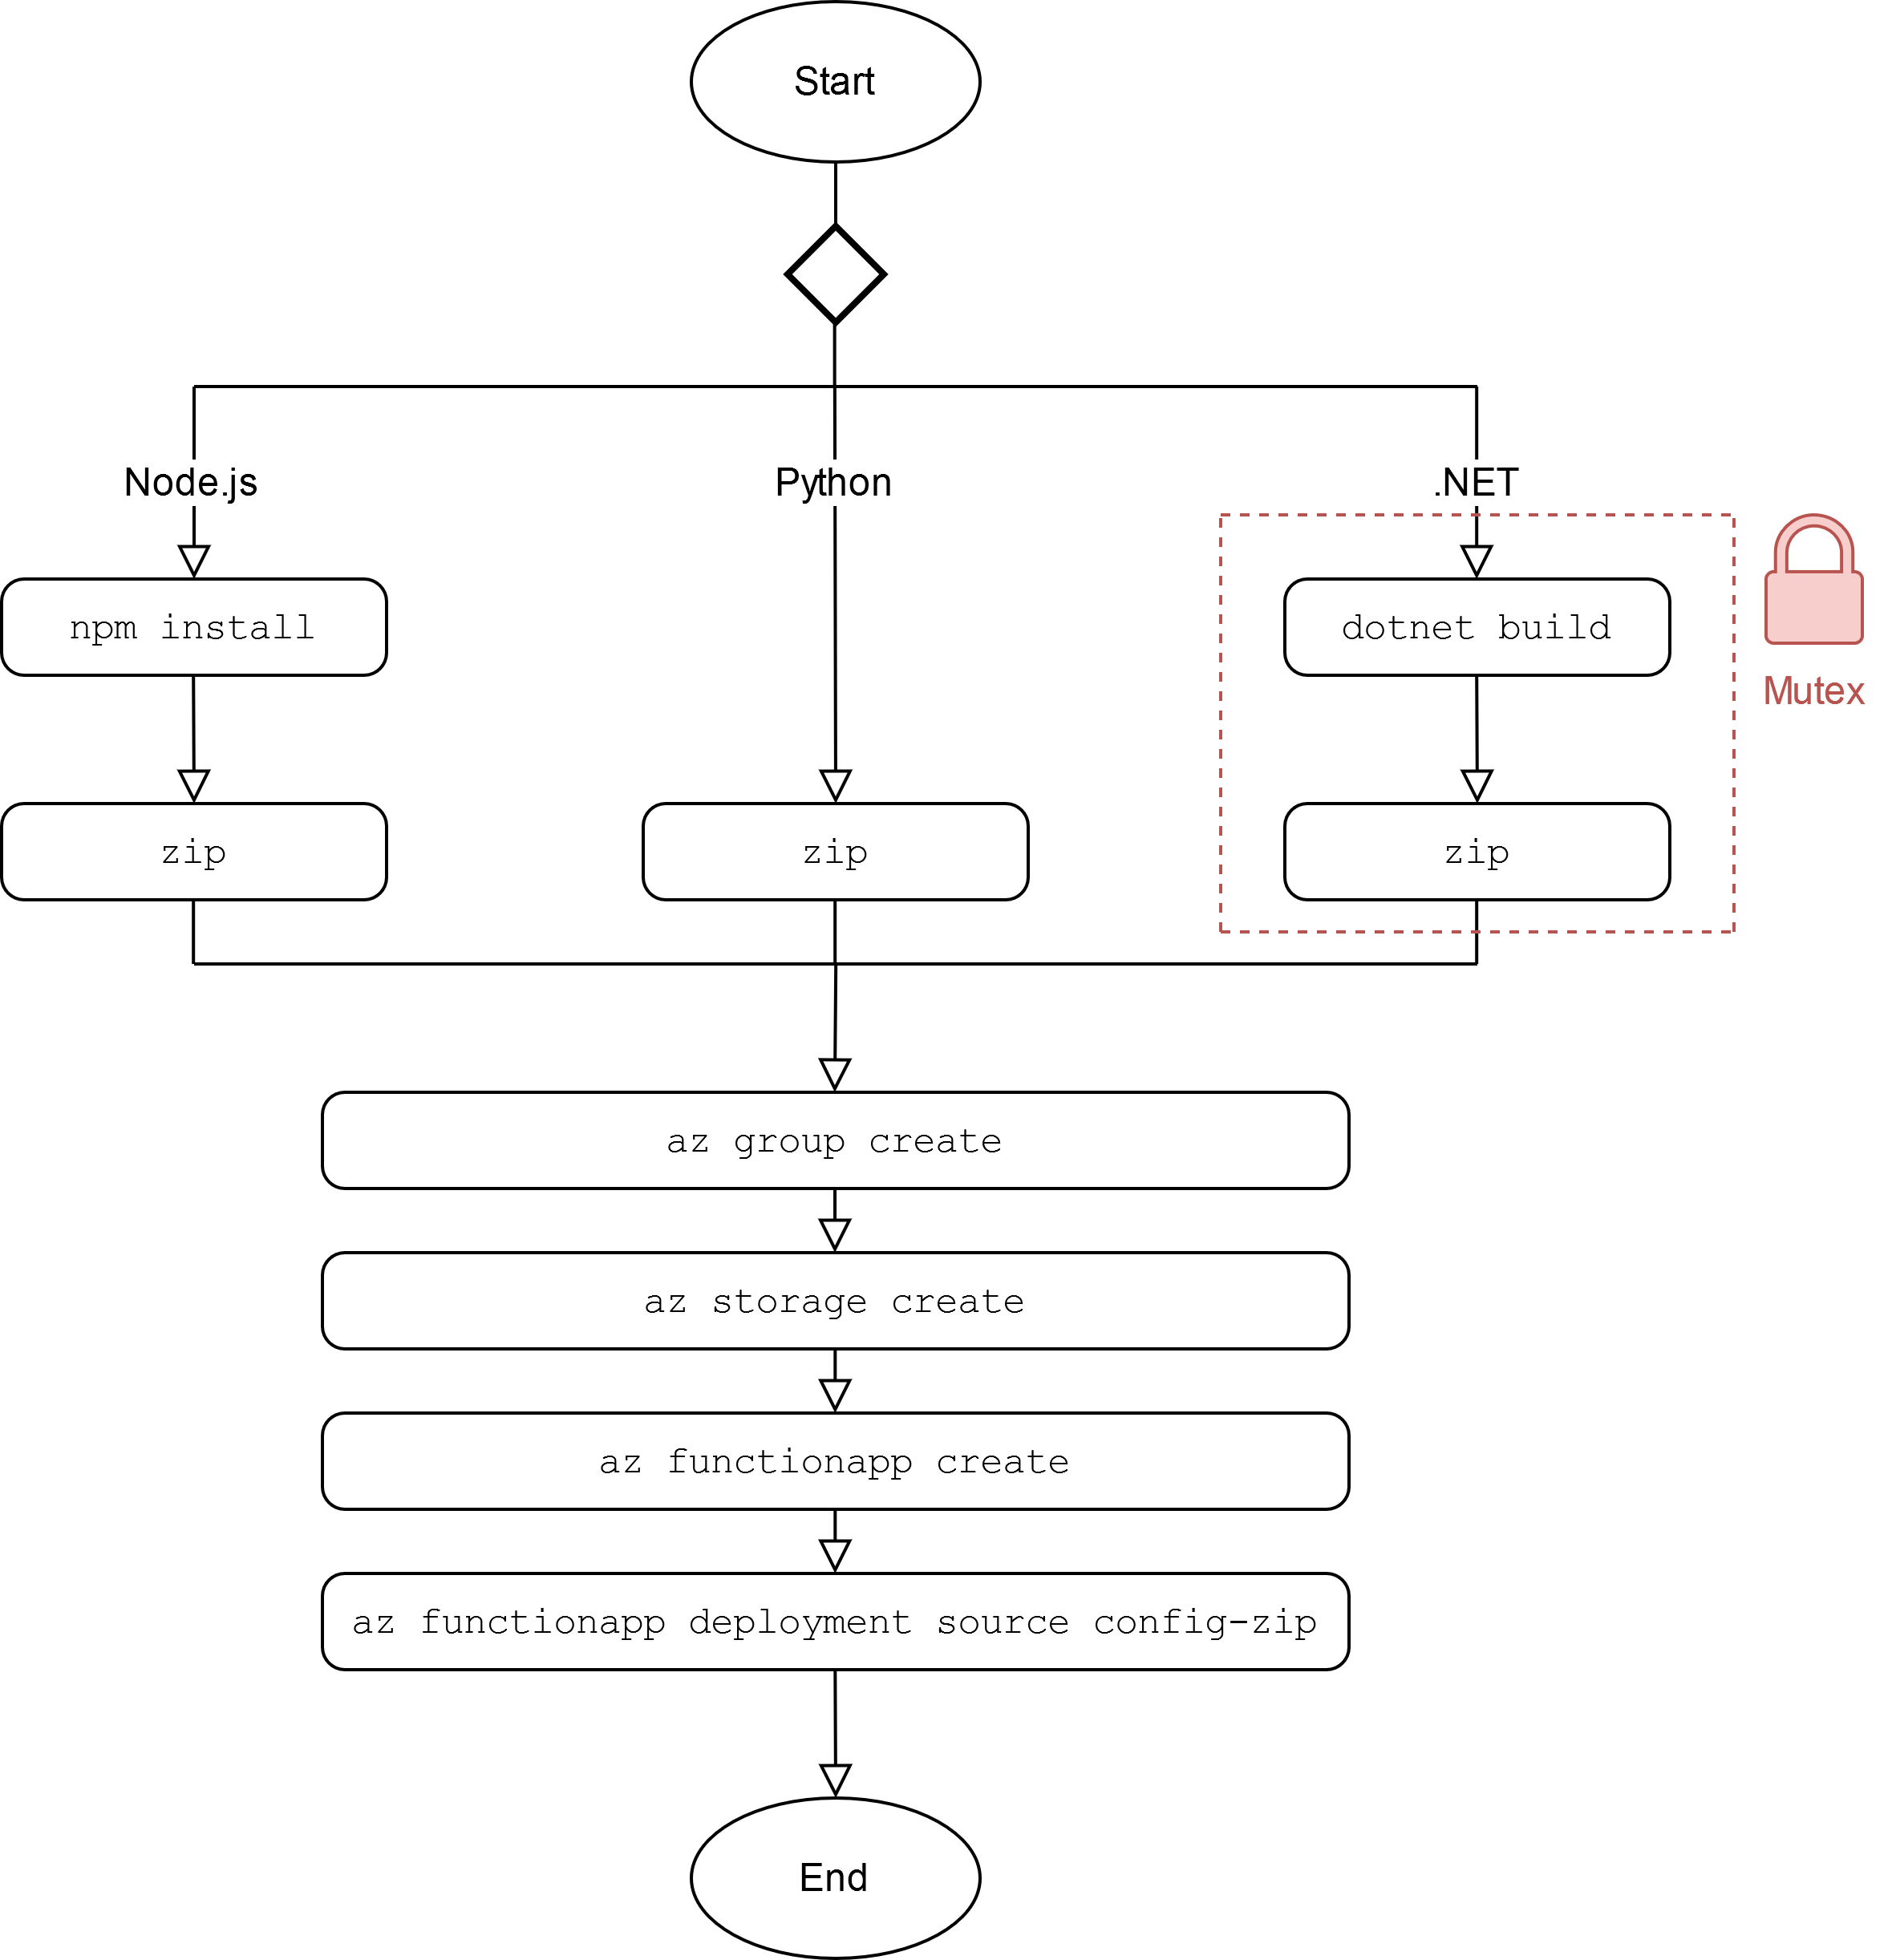
\includegraphics[width=0.8\textwidth]{bilder/Azure_Deploy_Flow.png}
\captionsetup{justification=centering, labelfont=bf}
\caption[Azure deployment flow chart]{Azure deployment flow chart\\Source: illustration by author}
\label{fig:azure_deploy}
\end{center}
\end{figure}

\begin{figure}[htp]
\begin{center}
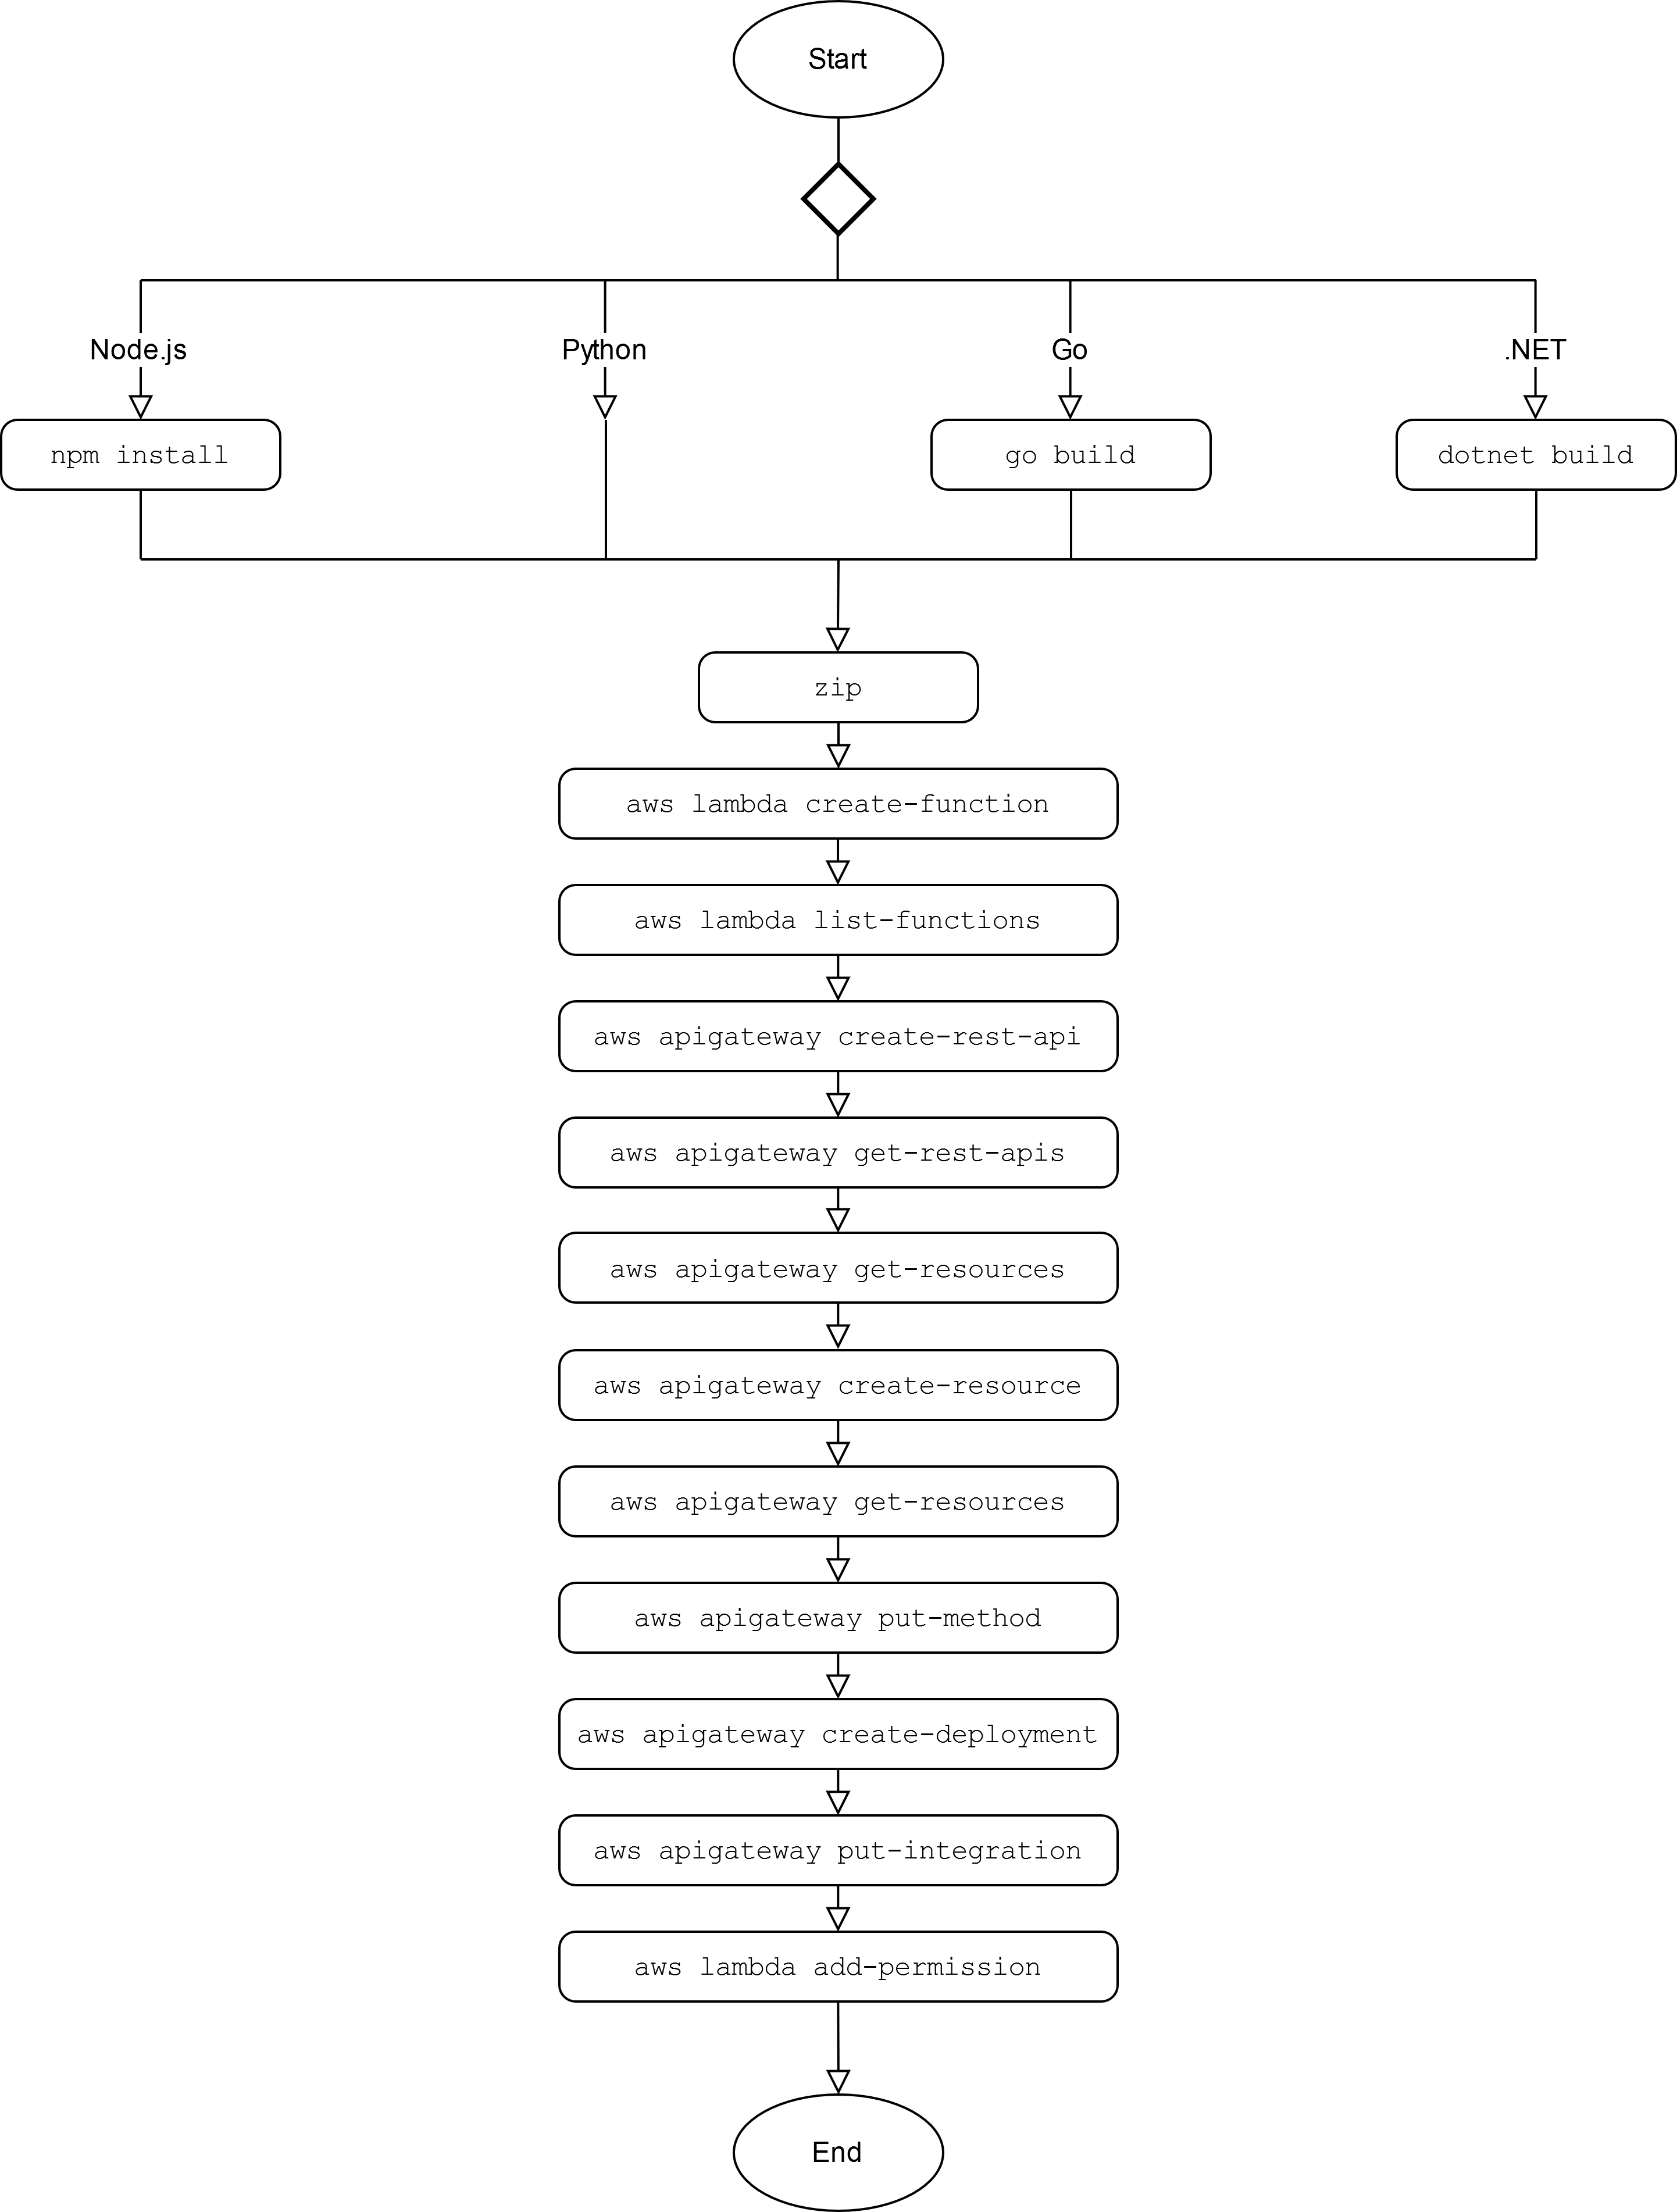
\includegraphics[width=0.8\textwidth]{bilder/AWS_Deploy_Flow.png}
\captionsetup{justification=centering, labelfont=bf}
\caption[AWS deployment flow chart]{AWS deployment flow chart\\Source: illustration by author}
\label{fig:aws_deploy}
\end{center}
\end{figure}

\begin{figure}[htp]
\begin{center}
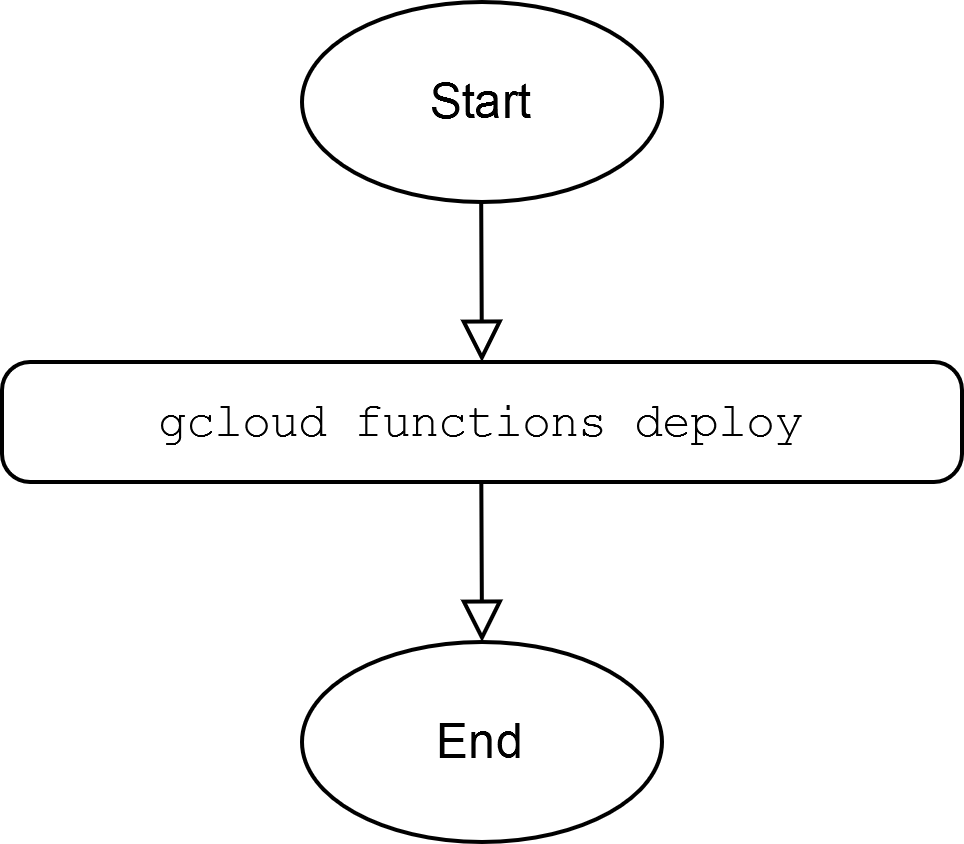
\includegraphics[width=0.3\textwidth]{bilder/Google_Deploy_Flow.png}
\captionsetup{justification=centering, labelfont=bf}
\caption[Google deployment flow chart]{Google deployment flow chart\\Source: illustration by author}
\label{fig:google_deploy}
\end{center}
\end{figure}

\begin{figure}[htp]
\begin{center}
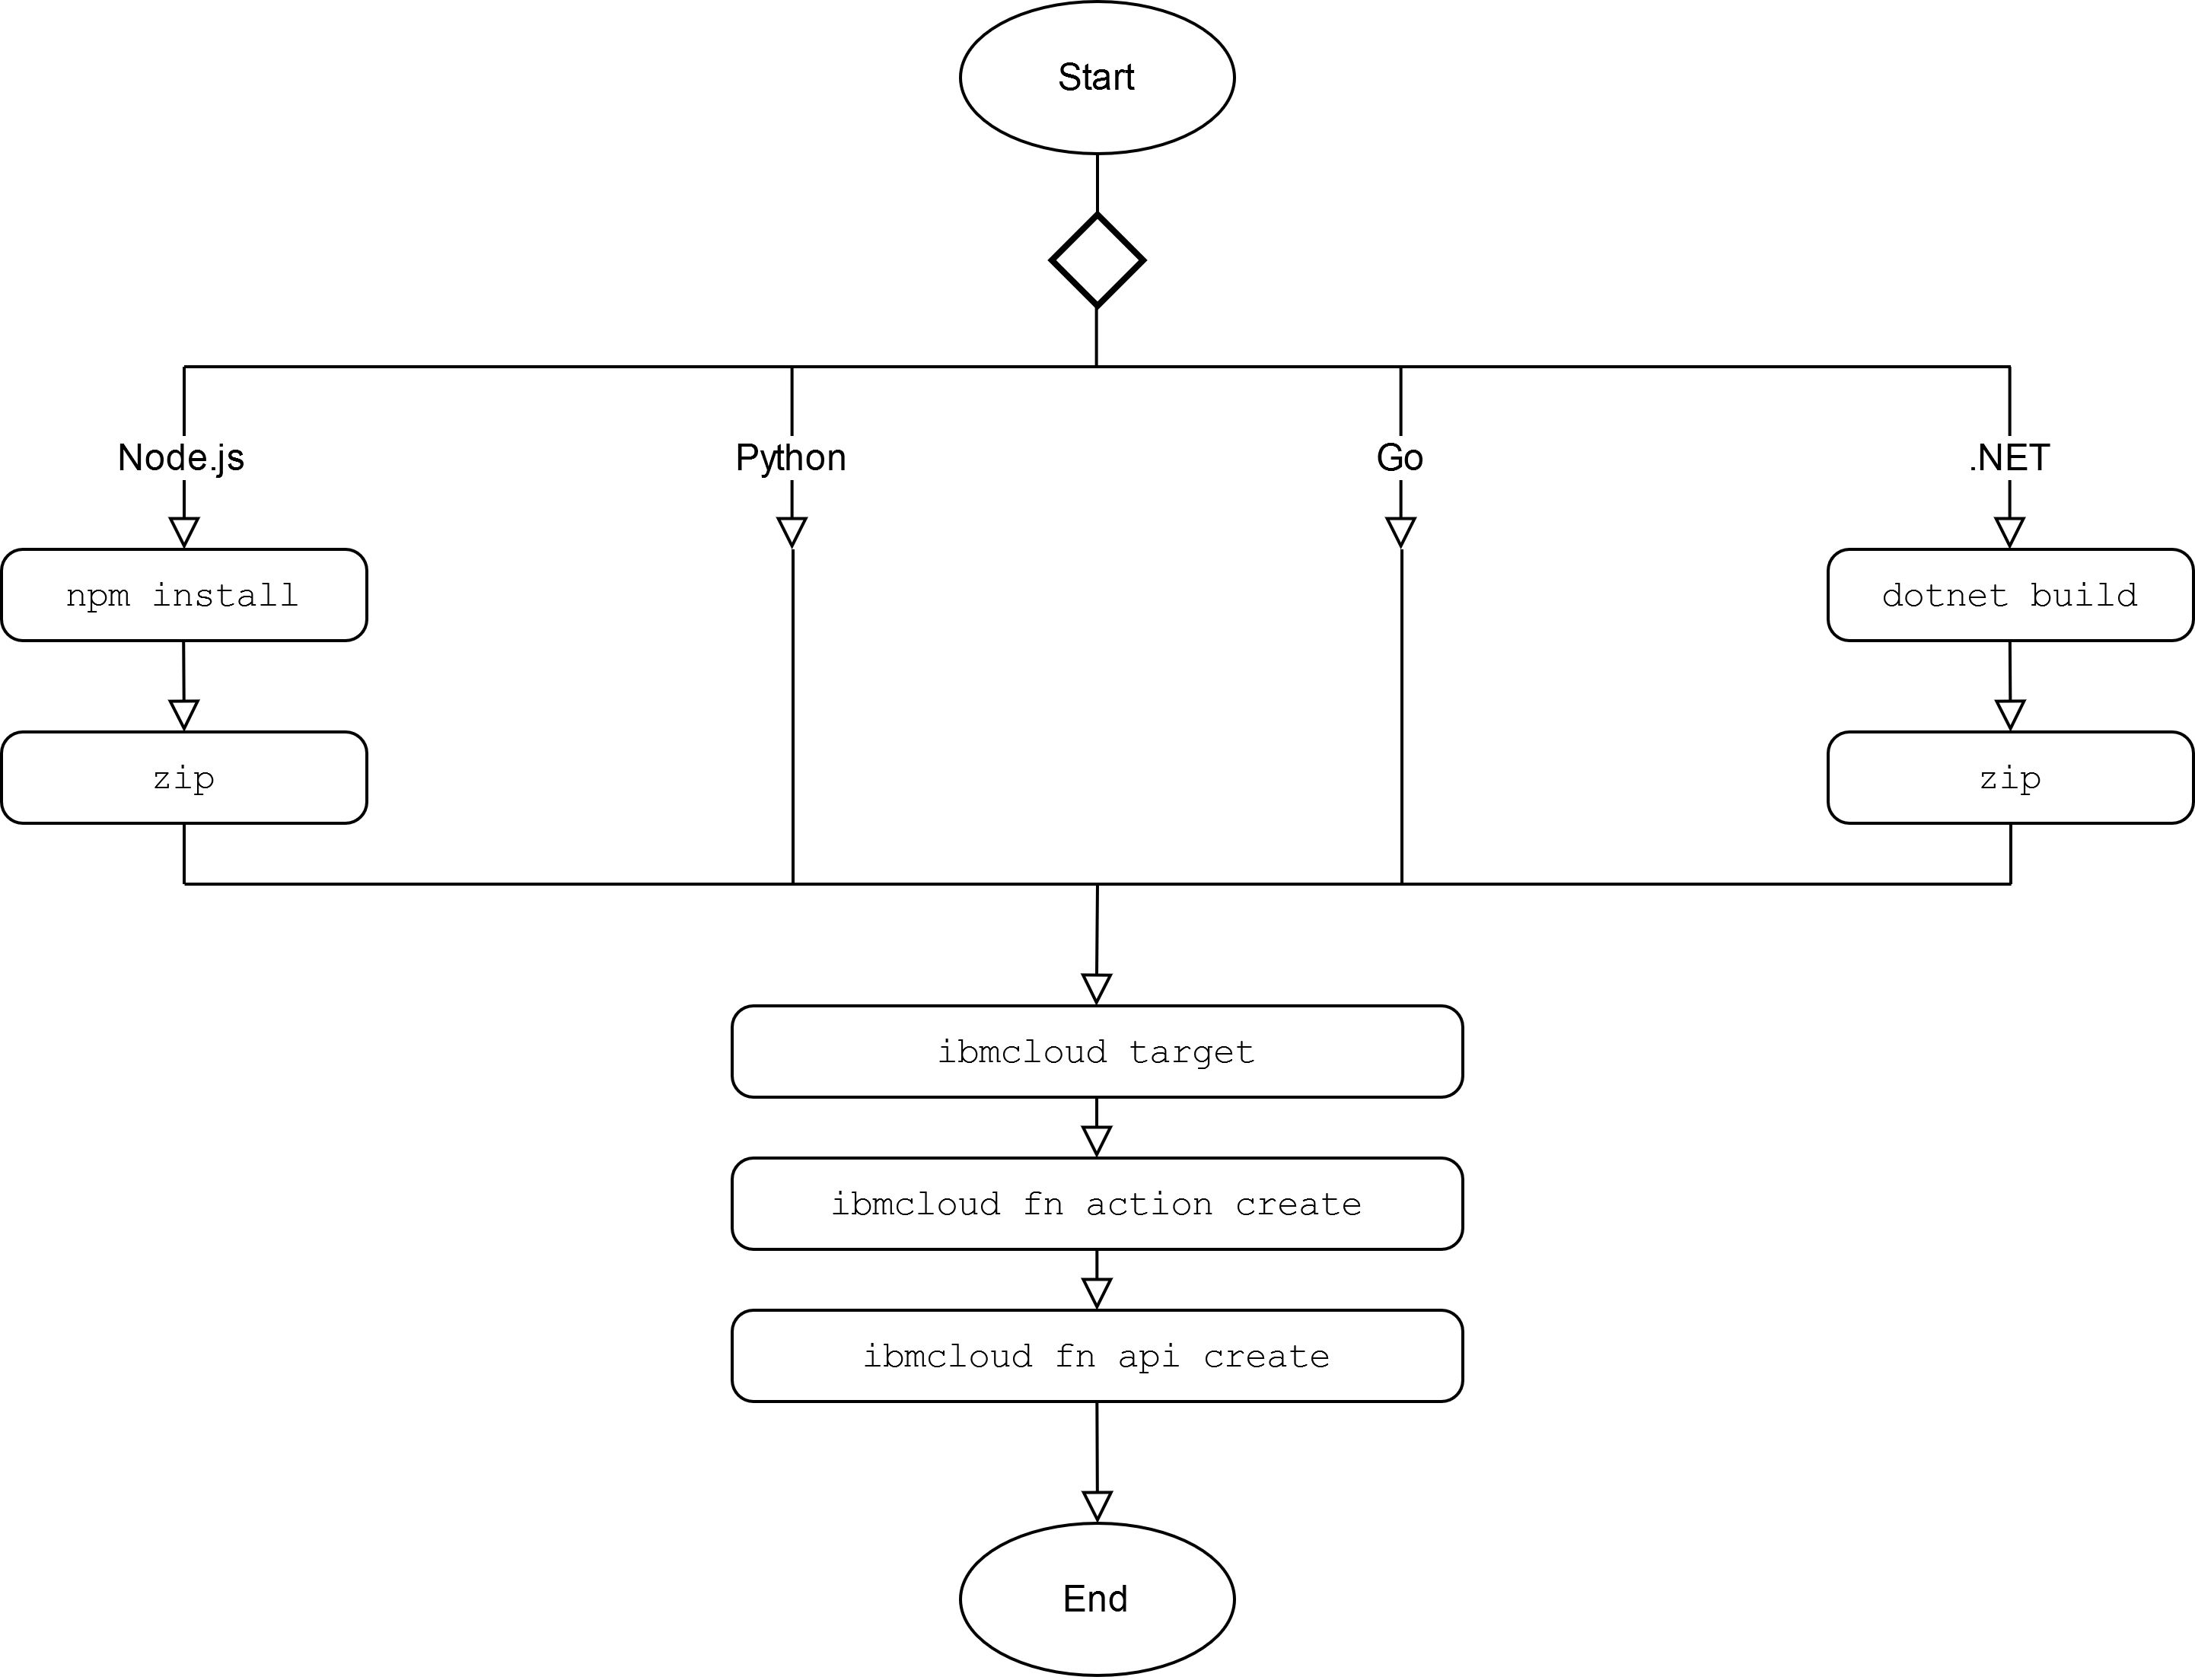
\includegraphics[width=0.8\textwidth]{bilder/IBM_Deploy_Flow.png}
\captionsetup{justification=centering, labelfont=bf}
\caption[IBM deployment flow chart]{IBM deployment flow chart\\Source: illustration by author}
\label{fig:ibm_deploy}
\end{center}
\end{figure}

\begin{figure}[htp]
\begin{center}
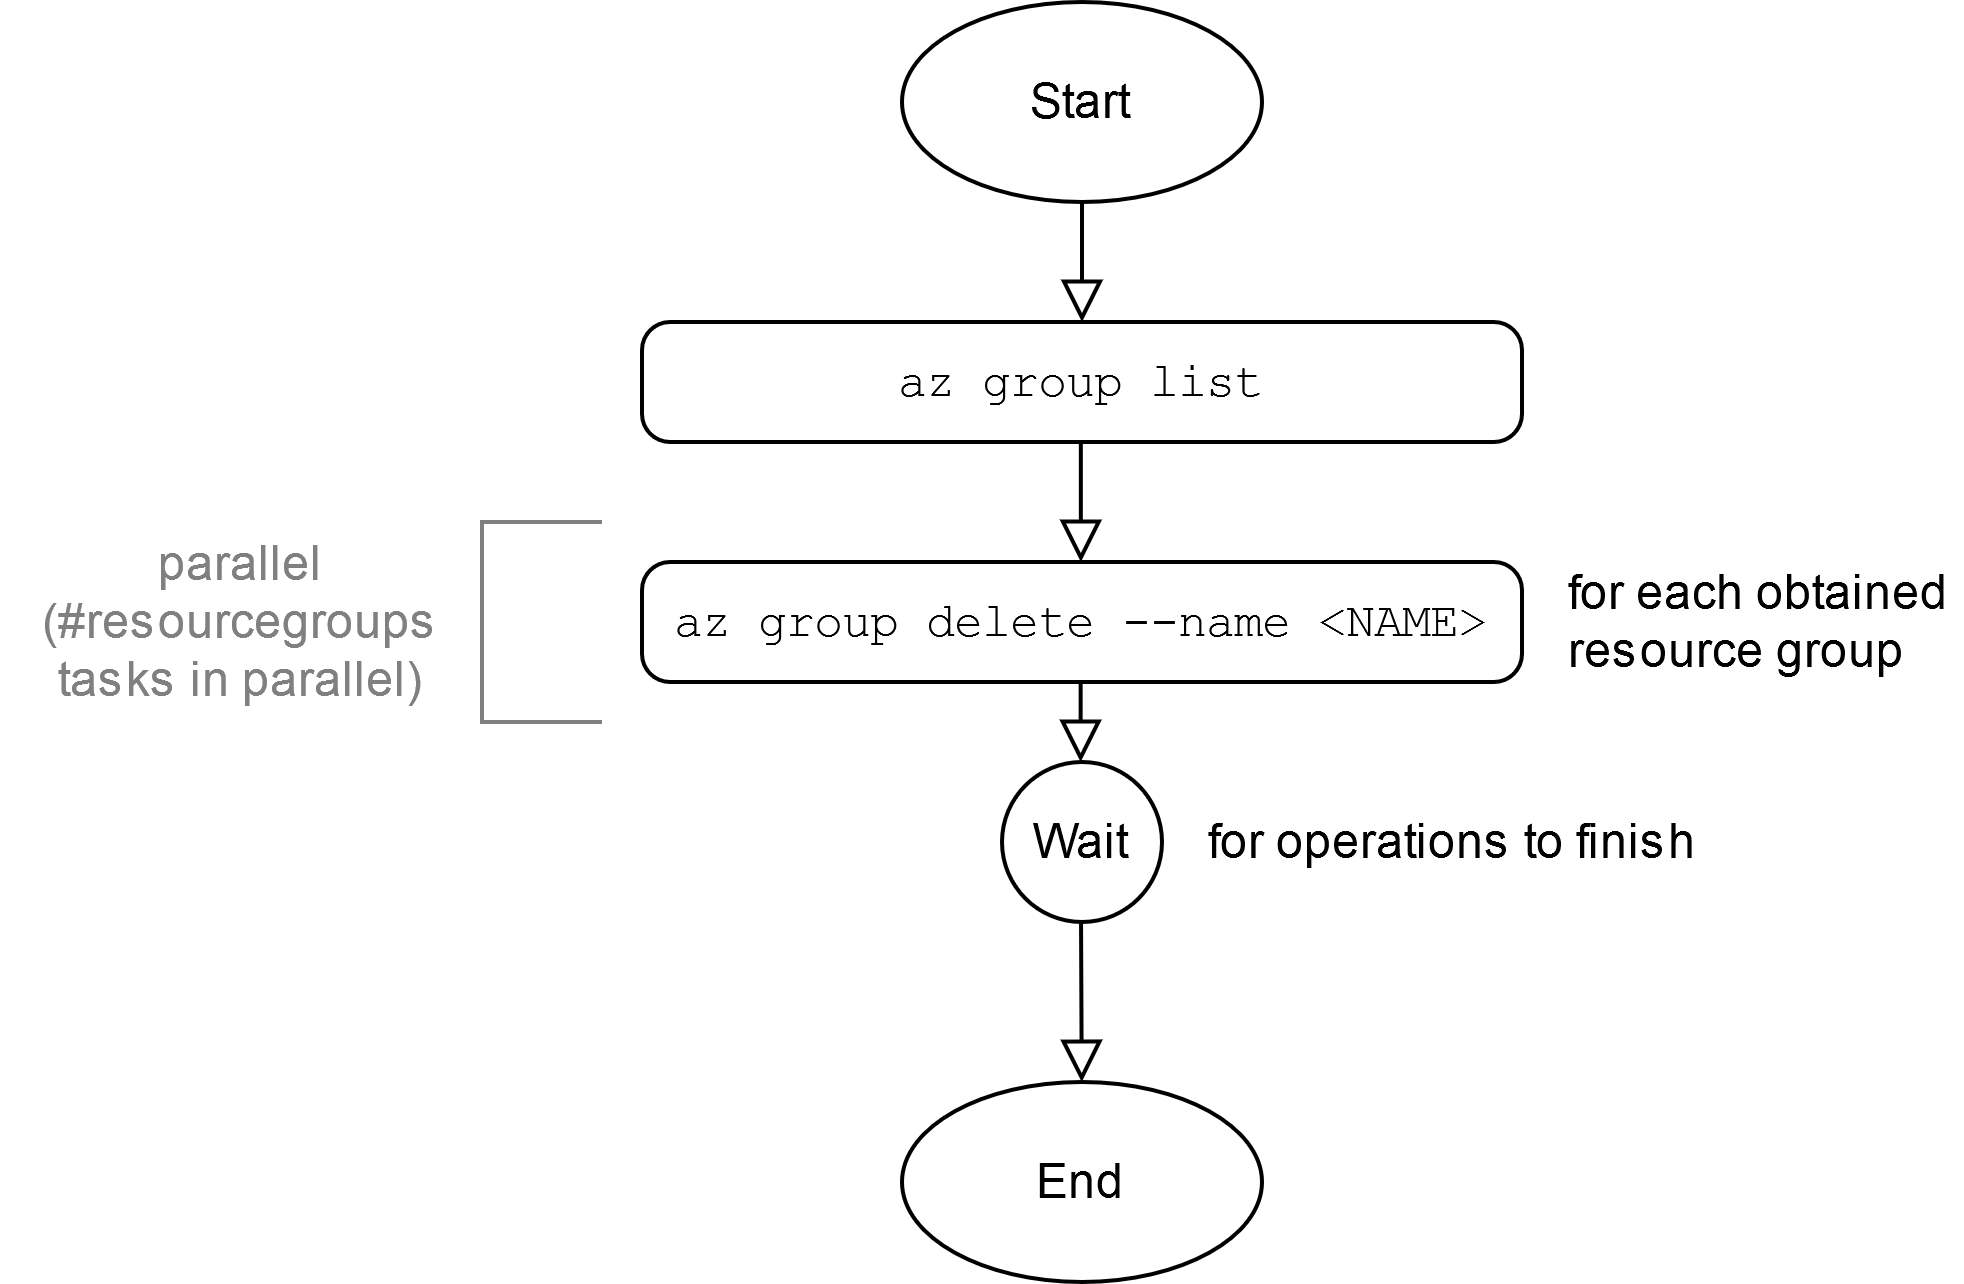
\includegraphics[width=0.7\textwidth]{bilder/Azure_Cleanup_Flow.png}
\captionsetup{justification=centering, labelfont=bf}
\caption[Azure cleanup flow chart]{Azure cleanup flow chart\\Source: illustration by author}
\label{fig:azure_cleanup}
\end{center}
\end{figure}

\begin{figure}[htp]
\begin{center}
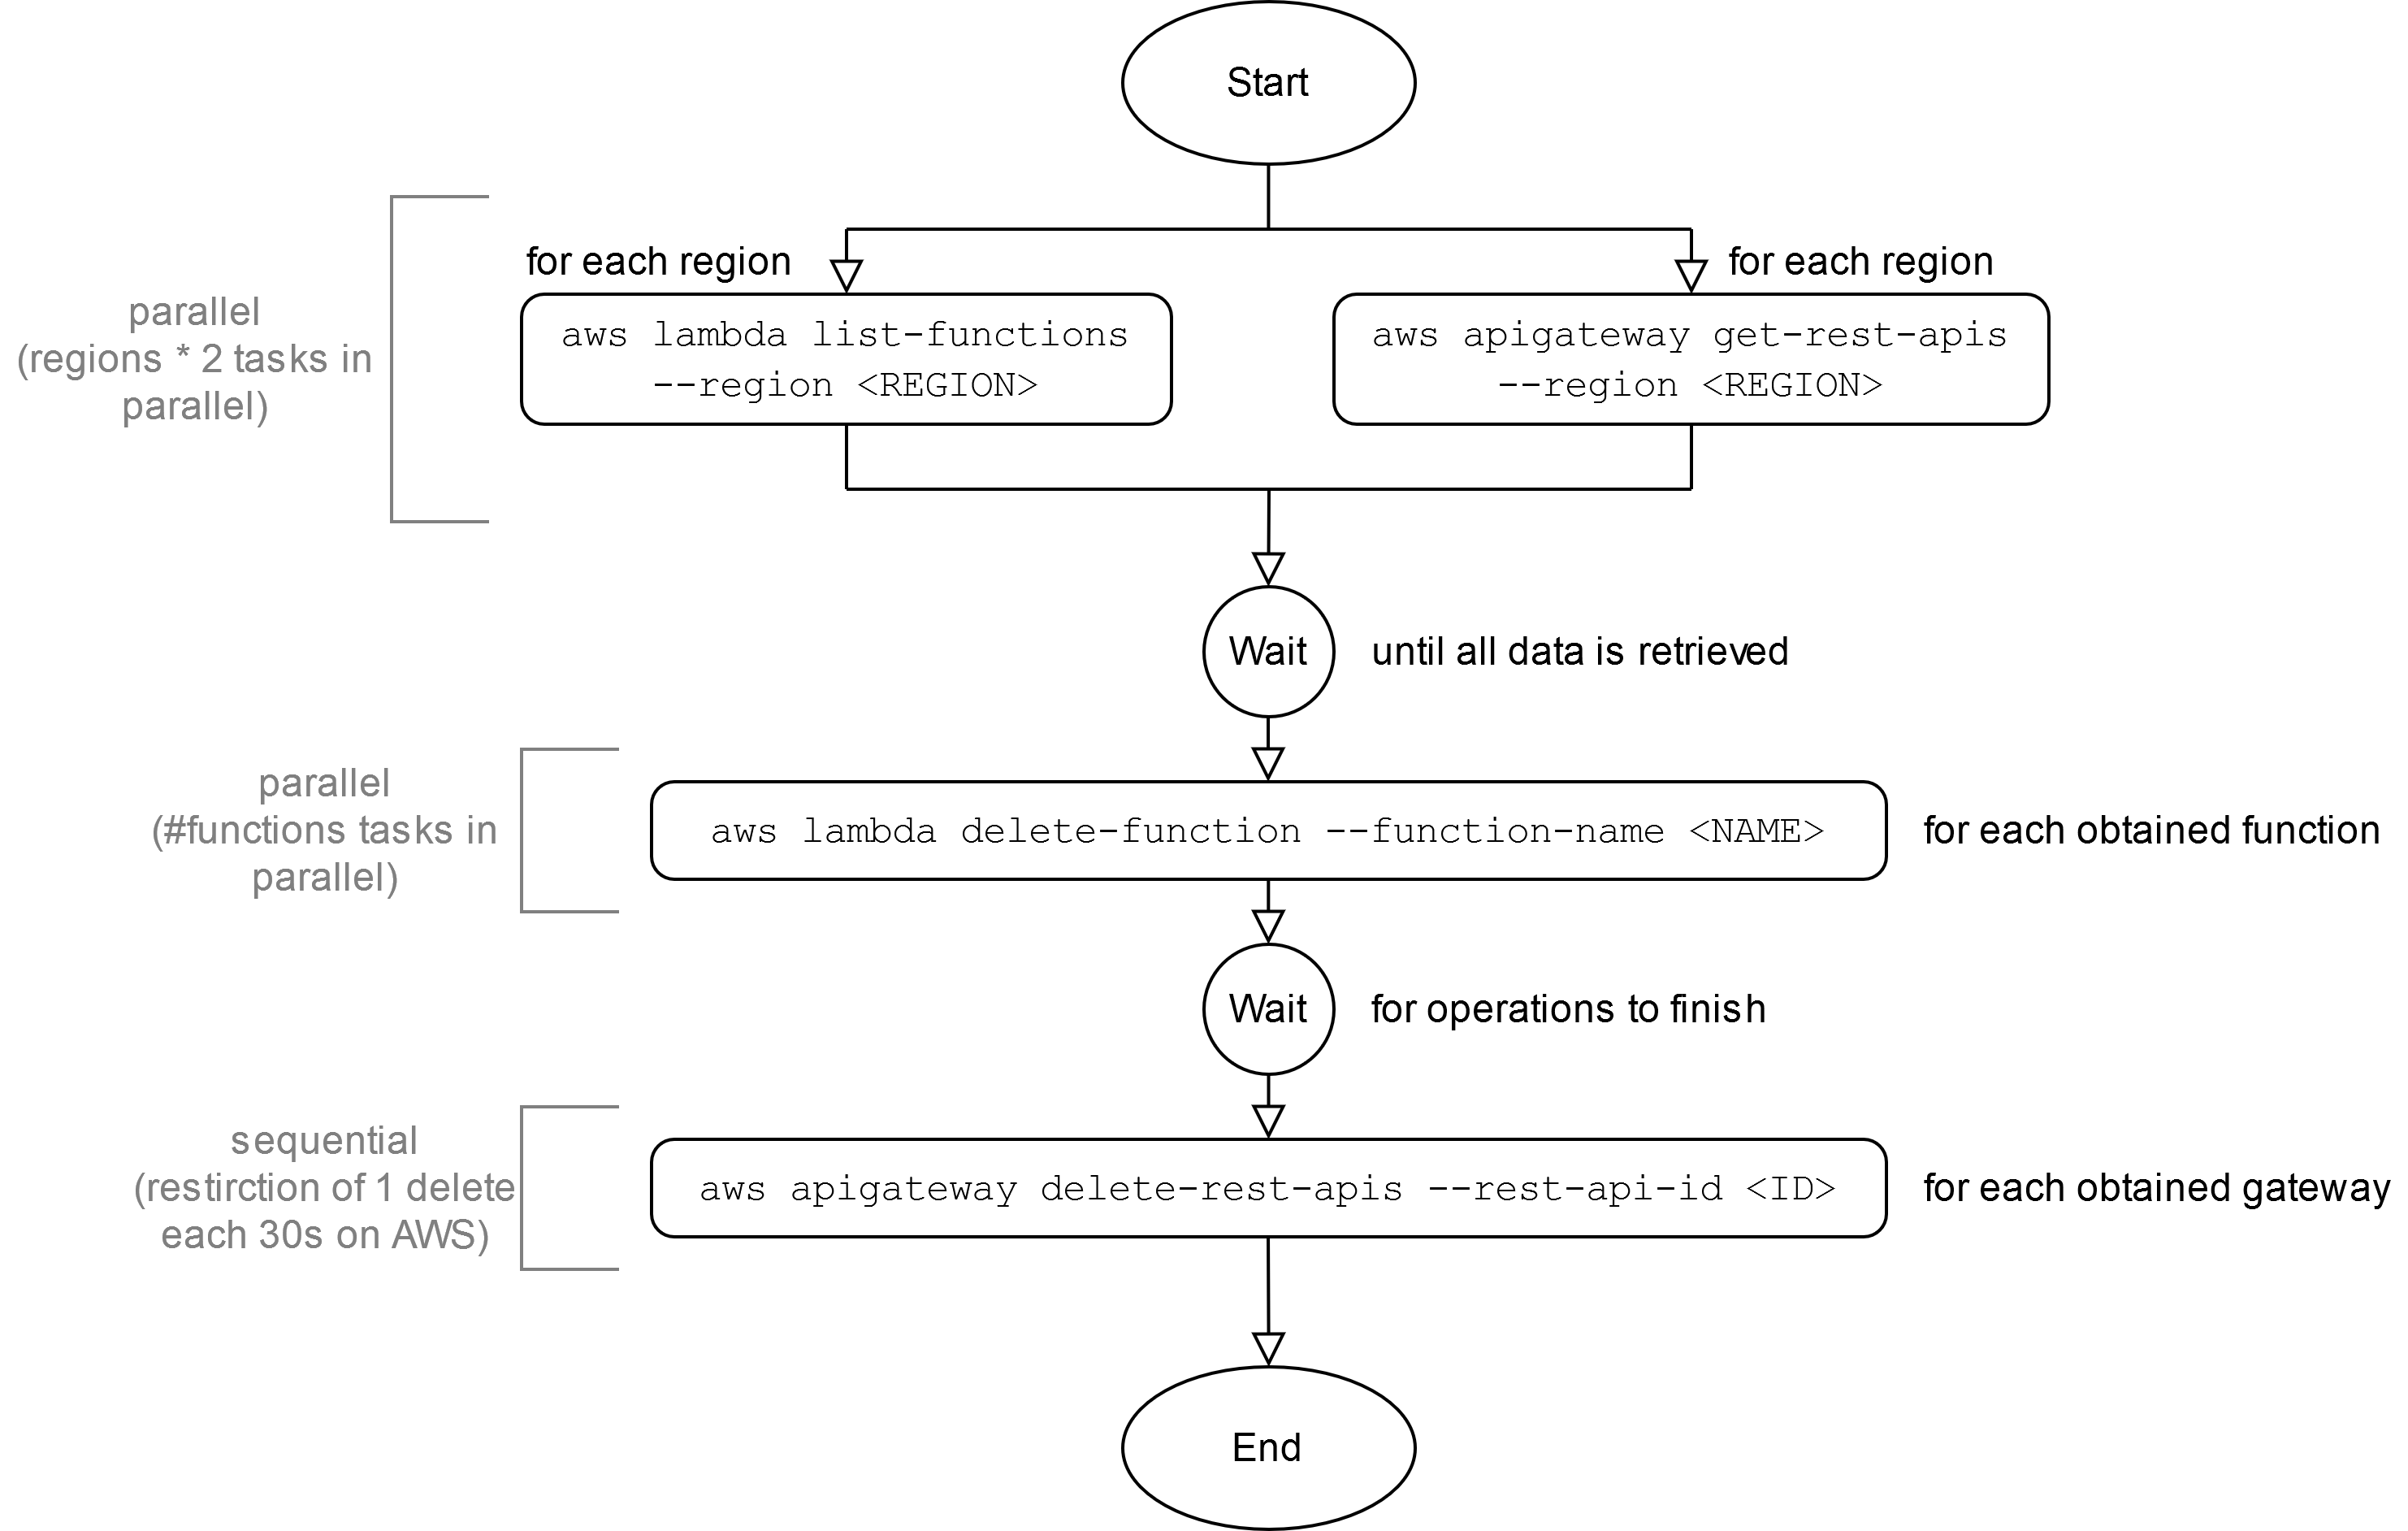
\includegraphics[width=0.9\textwidth]{bilder/AWS_Cleanup_Flow.png}
\captionsetup{justification=centering, labelfont=bf}
\caption[AWS cleanup flow chart]{AWS cleanup flow chart\\Source: illustration by author}
\label{fig:aws_cleanup}
\end{center}
\end{figure}

\begin{figure}[htp]
\begin{center}
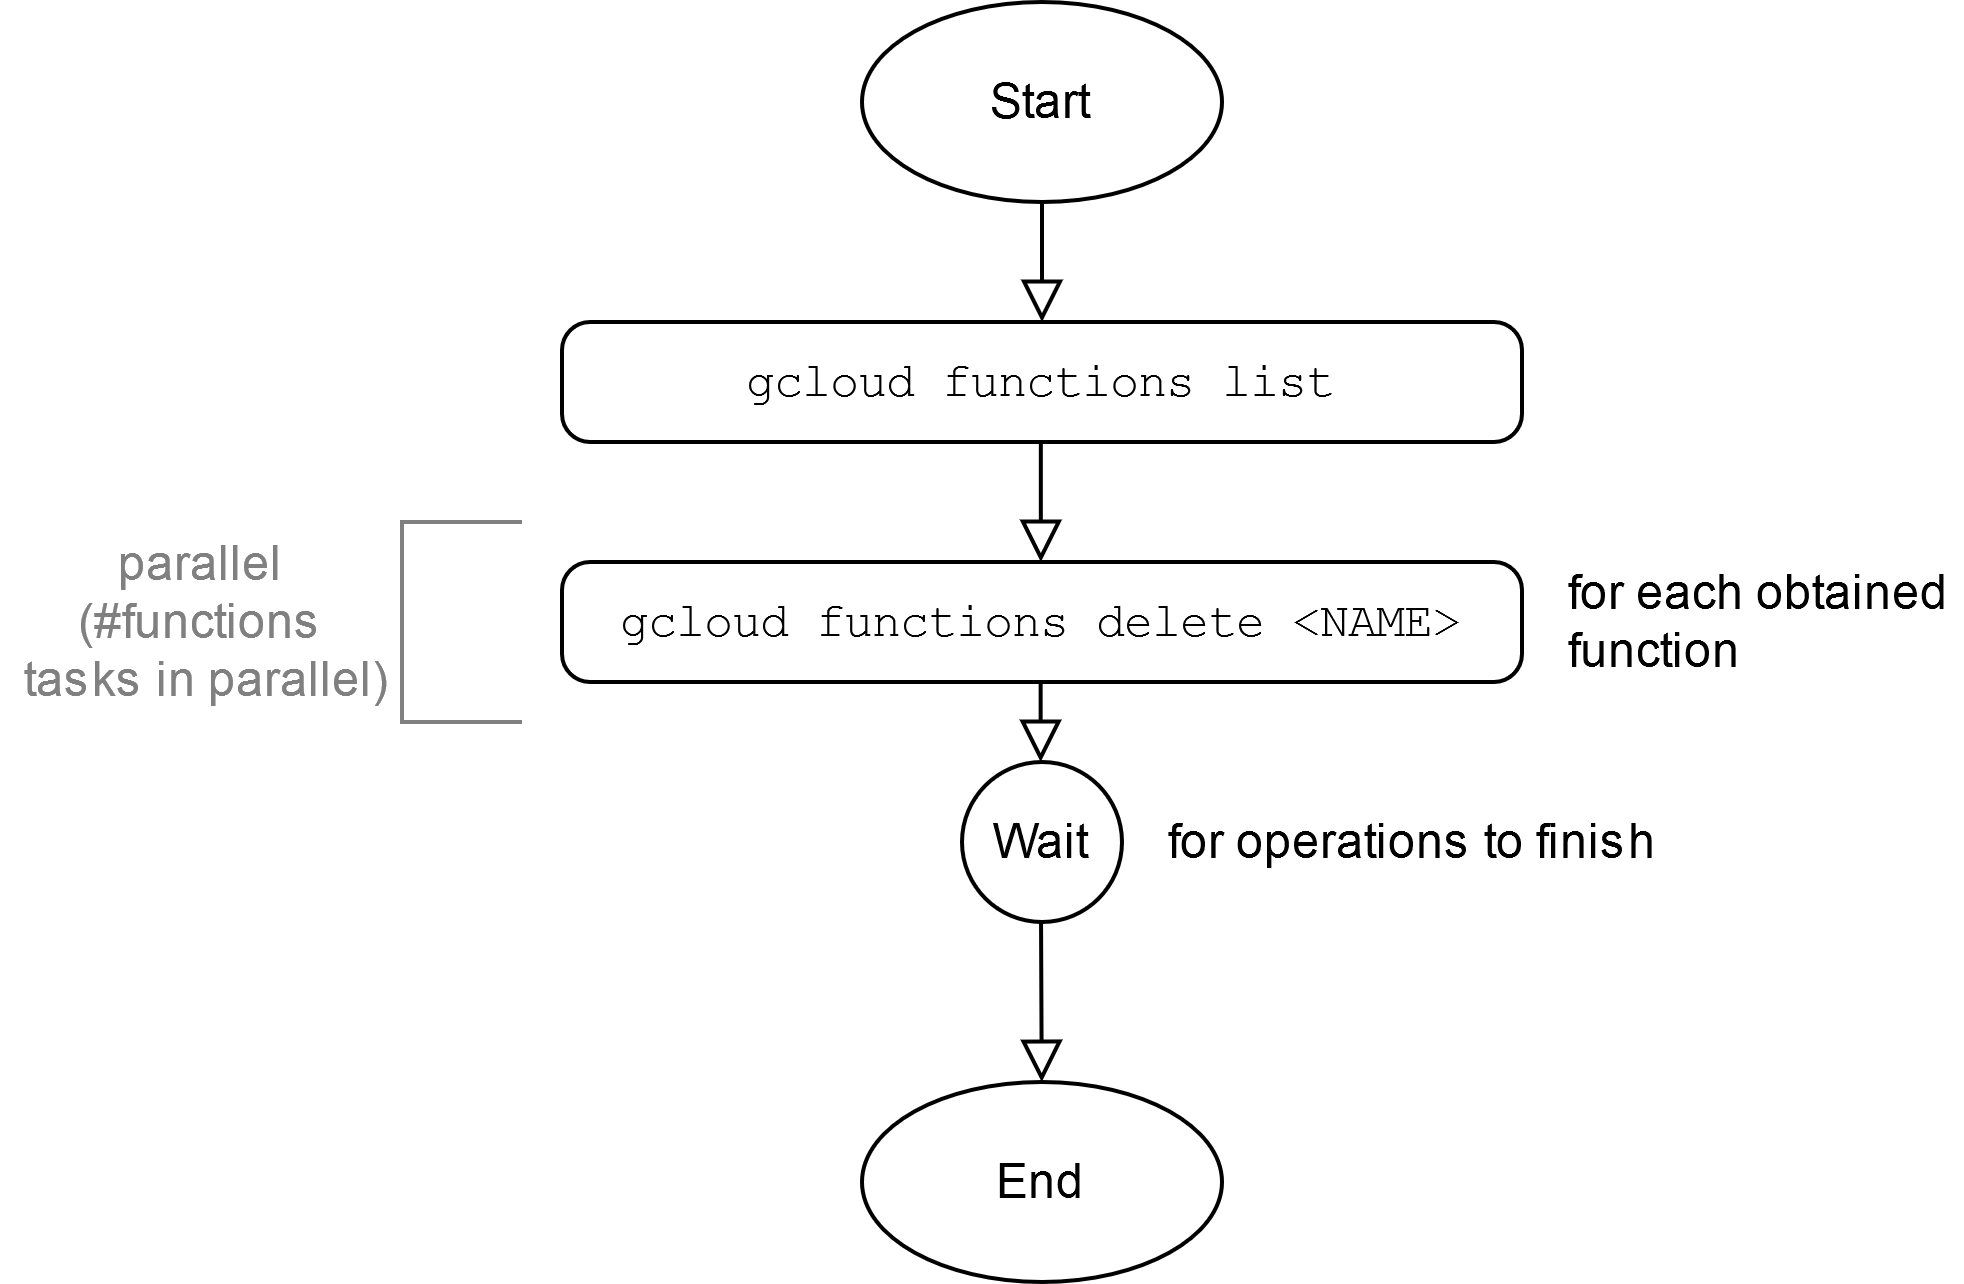
\includegraphics[width=0.6\textwidth]{bilder/Google_Cleanup_Flow.png}
\captionsetup{justification=centering, labelfont=bf}
\caption[Google cleanup flow chart]{Google cleanup flow chart\\Source: illustration by author}
\label{fig:google_cleanup}
\end{center}
\end{figure}

\begin{figure}[htp]
\begin{center}
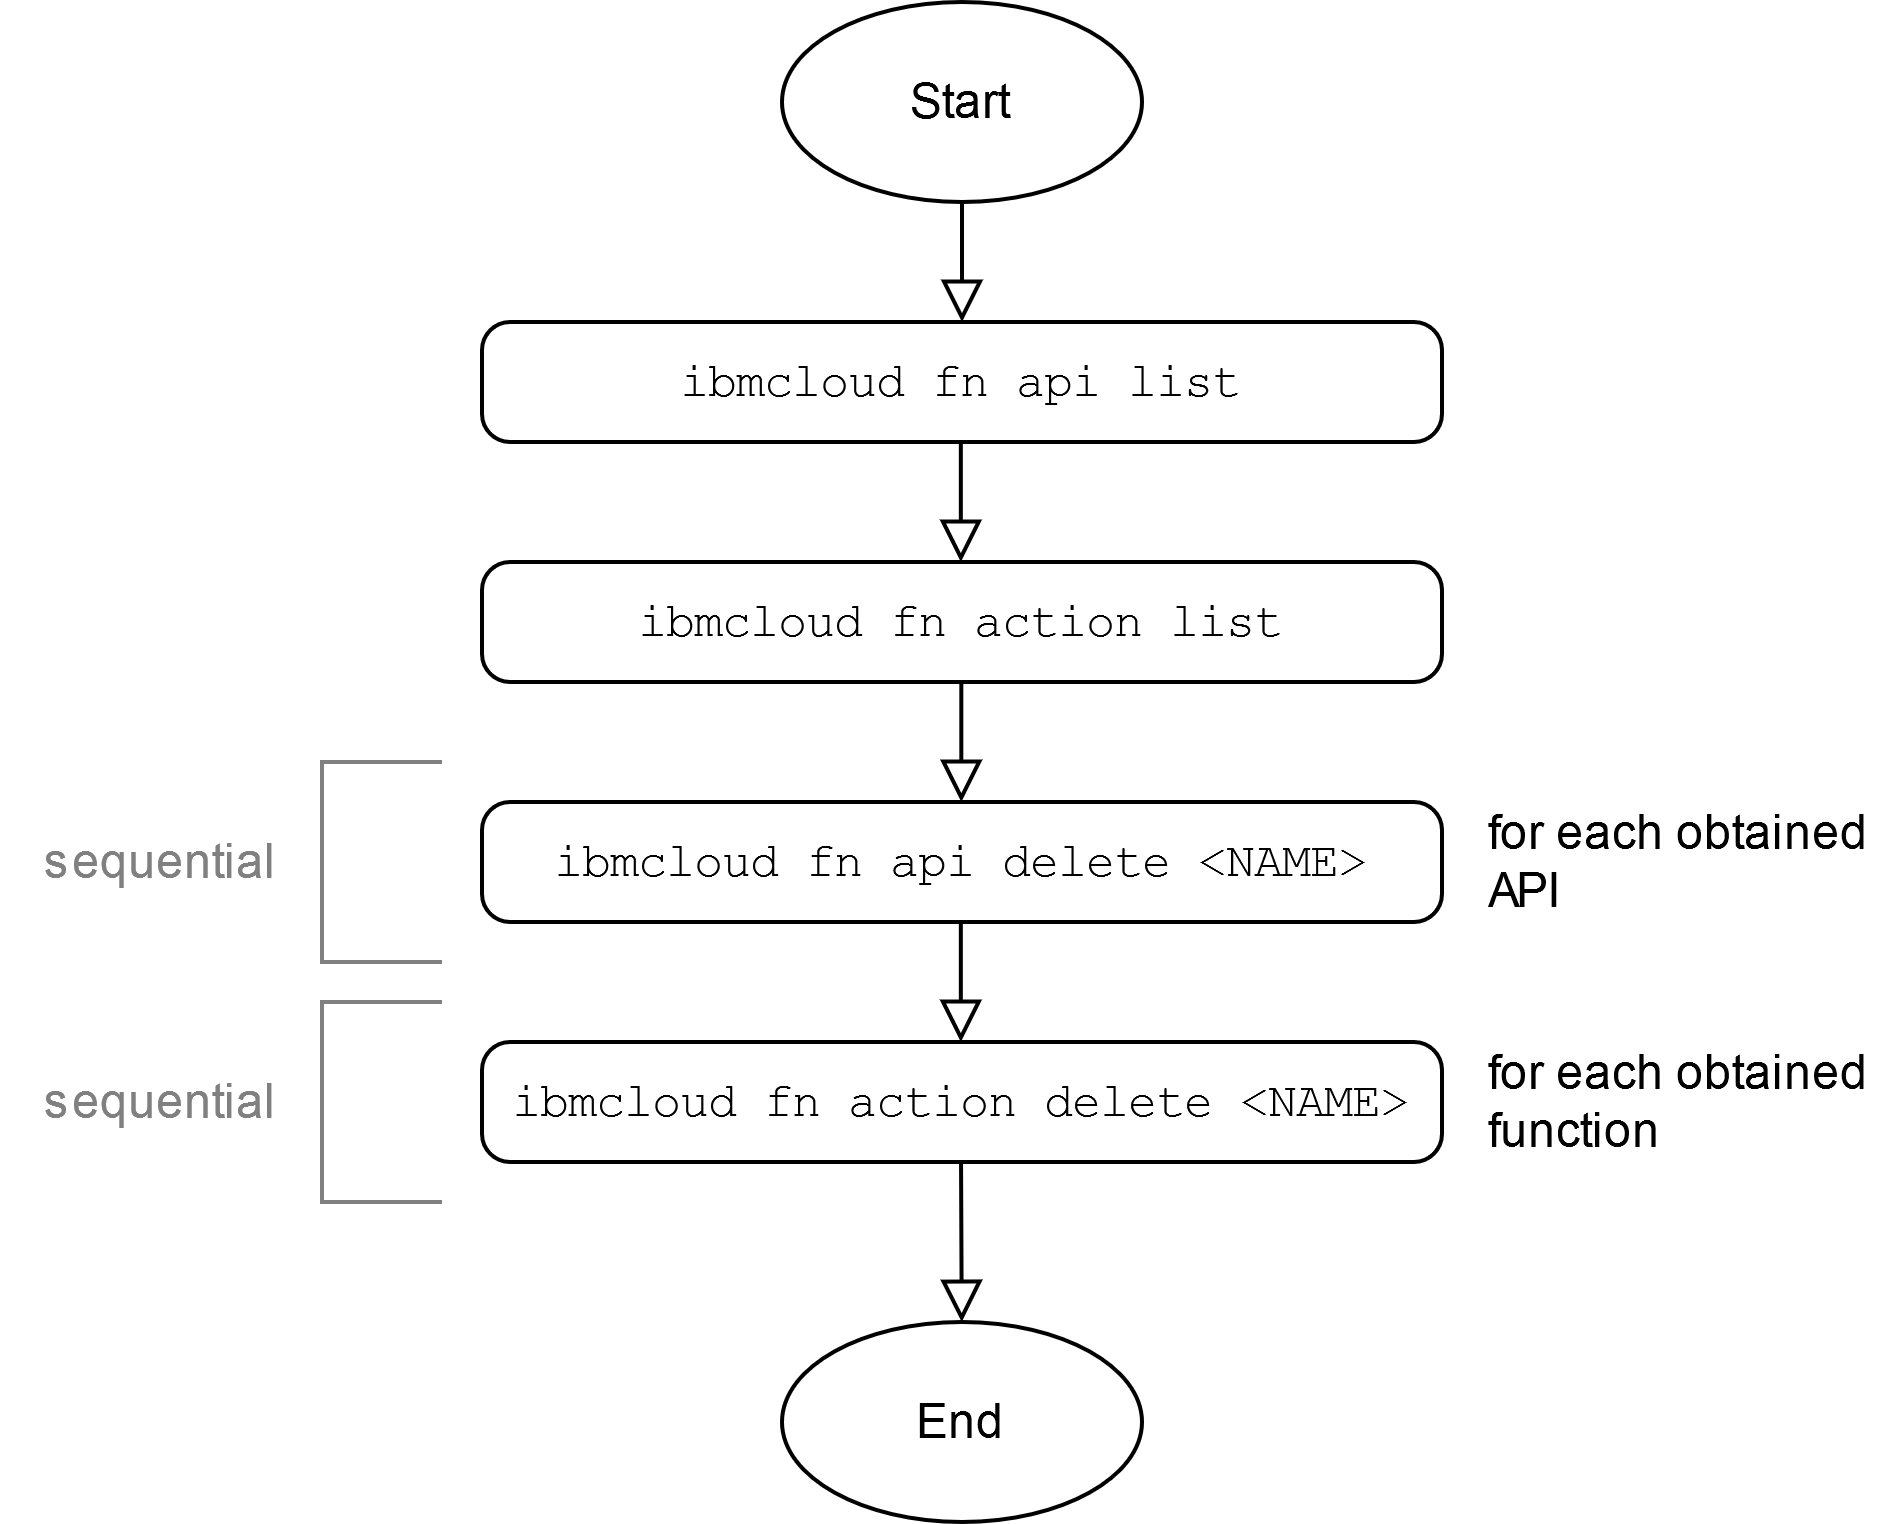
\includegraphics[width=0.6\textwidth]{bilder/IBM_Cleanup_Flow.png}
\captionsetup{justification=centering, labelfont=bf}
\caption[IBM cleanup flow chart]{IBM cleanup flow chart\\Source: illustration by author}
\label{fig:ibm_cleanup}
\end{center}
\end{figure}

\chapter{Results}
\begin{table}[h]
    \centering
    \renewcommand{\arraystretch}{0.9}
    \scalebox{0.8}{
    \begin{tabular}{|l|l|r|r|r|r|r|r|r|} \hline
\textbf{Cloud}	&	\textbf{Region}	&	\textbf{Dist. (km)}	&	\textbf{Avg.}	&	\textbf{Min.}	&	\textbf{Max.}	&	\textbf{Median}	&	\textbf{Q\textsubscript{1}}	&	\textbf{Q\textsubscript{3}}	\\	\hline
AWS	&	eu-central-1	&	365	&	80	&	51	&	328	&	77	&	67	&	88	\\	\hline
IBM	&	eu-de	&	365	&	205	&	97	&	2162	&	160	&	149	&	189	\\	\hline
AWS	&	eu-west-3	&	435	&	128	&	69	&	415	&	125	&	104	&	144	\\	\hline
Google	&	europe-west1	&	471	&	111	&	52	&	329	&	98	&	76	&	133	\\	\hline
Azure	&	westeurope	&	630	&	190	&	109	&	758	&	181	&	159	&	208	\\	\hline
AWS	&	eu-west-2	&	747	&	144	&	76	&	378	&	146	&	110	&	168	\\	\hline
Azure	&	uksouth	&	747	&	208	&	111	&	774	&	194	&	157	&	234	\\	\hline
Google	&	europe-west2	&	747	&	182	&	53	&	571	&	186	&	134	&	223	\\	\hline
IBM	&	eu-gb	&	747	&	227	&	124	&	1121	&	221	&	202	&	233	\\	\hline
AWS	&	eu-west-1	&	1290	&	170	&	87	&	377	&	176	&	161	&	190	\\	\hline
Azure	&	northeurope	&	1290	&	245	&	129	&	716	&	220	&	197	&	273	\\	\hline
AWS	&	eu-north-1	&	1544	&	159	&	82	&	602	&	154	&	135	&	174	\\	\hline
AWS	&	me-south-1	&	4423	&	499	&	189	&	938	&	505	&	486	&	534	\\	\hline
AWS	&	ca-central-1	&	5477	&	356	&	160	&	653	&	397	&	193	&	421	\\	\hline
IBM	&	us-east	&	6600	&	478	&	173	&	1023	&	486	&	467	&	505	\\	\hline
AWS	&	ap-south-1	&	6622	&	315	&	151	&	522	&	366	&	186	&	390	\\	\hline
AWS	&	us-east-1	&	6721	&	311	&	146	&	481	&	355	&	185	&	371	\\	\hline
Azure	&	eastus	&	6721	&	511	&	331	&	1239	&	475	&	458	&	542	\\	\hline
Azure	&	eastus2	&	6721	&	547	&	356	&	1168	&	504	&	480	&	552	\\	\hline
Google	&	us-east4	&	6721	&	291	&	130	&	812	&	187	&	153	&	247	\\	\hline
Google	&	us-east1	&	7220	&	496	&	146	&	1241	&	308	&	176	&	795	\\	\hline
AWS	&	us-east-2	&	7225	&	364	&	155	&	484	&	388	&	376	&	398	\\	\hline
Google	&	us-central1	&	7439	&	222	&	152	&	762	&	203	&	177	&	254	\\	\hline
Azure	&	southcentralus	&	8371	&	600	&	434	&	1115	&	613	&	585	&	633	\\	\hline
IBM	&	us-south	&	8371	&	618	&	220	&	1308	&	611	&	590	&	660	\\	\hline
Azure	&	westus2	&	8508	&	728	&	517	&	1846	&	718	&	704	&	760	\\	\hline
AWS	&	us-west-2	&	8690	&	515	&	223	&	1048	&	585	&	569	&	599	\\	\hline
AWS	&	ap-northeast-2	&	8865	&	809	&	323	&	1628	&	873	&	856	&	893	\\	\hline
AWS	&	us-west-1	&	9284	&	468	&	209	&	1138	&	541	&	246	&	556	\\	\hline
Azure	&	westus	&	9284	&	703	&	668	&	1668	&	677	&	673	&	686	\\	\hline
AWS	&	ap-east-1	&	9402	&	640	&	246	&	1280	&	659	&	646	&	680	\\	\hline
Azure	&	eastasia	&	9402	&	791	&	586	&	912	&	800	&	789	&	840	\\	\hline
Google	&	asia-east2	&	9402	&	1771	&	318	&	2726	&	2006	&	1980	&	2050	\\	\hline
AWS	&	sa-east-1	&	9531	&	674	&	270	&	1223	&	726	&	708	&	749	\\	\hline
AWS	&	ap-northeast-1	&	9669	&	808	&	298	&	1818	&	797	&	775	&	818	\\	\hline
Google	&	asia-northeast1	&	9669	&	1502	&	284	&	1902	&	1691	&	1667	&	1721	\\	\hline
IBM	&	jp-tok	&	9669	&	1287	&	1145	&	2095	&	1240	&	1212	&	1272	\\	\hline
AWS	&	ap-southeast-1	&	10381	&	549	&	222	&	1169	&	555	&	544	&	569	\\	\hline
Azure	&	southeastasia	&	10381	&	735	&	571	&	1190	&	719	&	701	&	742	\\	\hline
AWS	&	ap-southeast-2	&	16663	&	893	&	356	&	1313	&	956	&	948	&	972	\\	\hline
Azure	&	australiaeast	&	16663	&	1304	&	1251	&	1889	&	1269	&	1258	&	1308	\\	\hline
    \end{tabular}}
    \caption[Latency test details]{Latency test details, all numbers in milliseconds except for distance, distances calculated with \href{https://www.distance.to/}{https://www.distance.to/}}
    \label{tab:latency}
\end{table}
\renewcommand{\arraystretch}{1}

\begin{table}[h]
    \centering
    \begin{tabular}{|l|l|r|r|r|r|r|r|} \hline
\textbf{Cloud}	&	\textbf{Runtime}	&	\textbf{Avg.}	&	\textbf{Min.}	&	\textbf{Max.}	&	\textbf{Median}	&	\textbf{Q\textsubscript{1}}	&	\textbf{Q\textsubscript{3}}	\\ \hline
AWS	&	Node.js	&	352	&	275	&	845	&	298	&	285	&	315	\\ \hline
AWS	&	Python	&	246	&	224	&	276	&	247	&	231	&	257	\\ \hline
AWS	&	Go	&	267	&	223	&	357	&	264	&	239	&	277	\\ \hline
AWS	&	.NET	&	1689	&	1539	&	1798	&	1701	&	1639	&	1739	\\ \hline
Azure	&	Node.js	&	2511	&	2275	&	2795	&	2482	&	2396	&	2630	\\ \hline
Azure	&	Python	&	3019	&	2325	&	4517	&	3026	&	2537	&	3138	\\ \hline
Azure	&	.NET	&	3637	&	2507	&	4937	&	3747	&	3131	&	3850	\\ \hline
Azure (Windows)	&	Node.js	&	4086	&	3226	&	4974	&	4046	&	3782	&	4358	\\ \hline
Azure (Windows)	&	.NET	&	1864	&	1256	&	3419	&	1635	&	1441	&	1897	\\ \hline
Google	&	Node.js	&	1933	&	1559	&	2294	&	1897	&	1691	&	2215	\\ \hline
Google	&	Python	&	2694	&	2160	&	3847	&	2482	&	2410	&	2784	\\ \hline
Google	&	Go	&	1613	&	1178	&	2067	&	1564	&	1487	&	1745	\\ \hline
IBM	&	Node.js	&	826	&	779	&	925	&	819	&	796	&	850	\\ \hline
IBM	&	Python	&	646	&	599	&	675	&	650	&	633	&	665	\\ \hline
IBM	&	Go	&	788	&	733	&	906	&	771	&	761	&	799	\\ \hline
IBM	&	.NET	&	1670	&	1583	&	1829	&	1672	&	1631	&	1685	\\ \hline
\end{tabular}
    \caption[Cold start test details]{Cold start test details, all numbers in milliseconds}
    \label{tab:latency}
\end{table}

\begin{table}[htp]
    \centering
    \renewcommand{\arraystretch}{0.9}
    \scalebox{0.9}{
    \begin{tabular}{|l|l|r|r|r|r|r|r|r|} \hline
\textbf{Cloud}	&	
\textbf{Runtime}	&	
\textbf{Memory}	&	
\textbf{Avg.}	&	
\textbf{Min.}	&	
\textbf{Max.}	&	
\textbf{Median}	&	
\textbf{Q\textsubscript{1}}	&	
\textbf{Q\textsubscript{3}}	\\ \hline
AWS	&	Node.js	&	128	&	17031	&	16454	&	18377	&	16816	&	16676	&	17101	\\ \hline
AWS	&	Node.js	&	256	&	8697	&	8199	&	9298	&	8552	&	8312	&	9143	\\ \hline
AWS	&	Node.js	&	512	&	4367	&	4233	&	4569	&	4319	&	4276	&	4462	\\ \hline
AWS	&	Node.js	&	1024	&	2078	&	2045	&	2118	&	2077	&	2065	&	2088	\\ \hline
AWS	&	Node.js	&	2048	&	1135	&	1113	&	1195	&	1132	&	1125	&	1139	\\ \hline
AWS	&	Python	&	128	&	7903	&	7809	&	8040	&	7903	&	7870	&	7927	\\ \hline
AWS	&	Python	&	256	&	3935	&	3890	&	4017	&	3928	&	3915	&	3942	\\ \hline
AWS	&	Python	&	512	&	1948	&	1915	&	1973	&	1947	&	1942	&	1955	\\ \hline
AWS	&	Python	&	1024	&	1000	&	981	&	1020	&	1000	&	996	&	1005	\\ \hline
AWS	&	Python	&	2048	&	564	&	550	&	591	&	566	&	555	&	571	\\ \hline
AWS	&	Go	&	128	&	934	&	848	&	1004	&	940	&	912	&	960	\\ \hline
AWS	&	Go	&	256	&	454	&	412	&	487	&	460	&	442	&	465	\\ \hline
AWS	&	Go	&	512	&	221	&	196	&	237	&	220	&	216	&	228	\\ \hline
AWS	&	Go	&	1024	&	103	&	91	&	112	&	104	&	99	&	107	\\ \hline
AWS	&	Go	&	2048	&	63	&	62	&	70	&	63	&	63	&	63	\\ \hline
AWS	&	.NET	&	128	&	669	&	631	&	716	&	666	&	658	&	679	\\ \hline
AWS	&	.NET	&	256	&	330	&	306	&	364	&	331	&	323	&	336	\\ \hline
AWS	&	.NET	&	512	&	160	&	146	&	180	&	159	&	155	&	163	\\ \hline
AWS	&	.NET	&	1024	&	80	&	74	&	88	&	79	&	78	&	83	\\ \hline
AWS	&	.NET	&	2048	&	51	&	50	&	64	&	50	&	50	&	50	\\ \hline
Azure	&	Node.js	&	1536	&	2157	&	1993	&	2552	&	2134	&	2064	&	2227	\\ \hline
Azure	&	Python	&	1536	&	1267	&	1167	&	1764	&	1227	&	1205	&	1299	\\ \hline
Azure	&	.NET	&	1536	&	92	&	80	&	127	&	89	&	87	&	95	\\ \hline
AzureWindows	&	Node.js	&	1536	&	6157	&	5190	&	12717	&	5748	&	5309	&	6426	\\ \hline
AzureWindows	&	.NET	&	1536	&	253	&	231	&	400	&	250	&	245	&	254	\\ \hline
Google	&	Node.js	&	128	&	16535	&	2822	&	25818	&	15900	&	14923	&	18535	\\ \hline
Google	&	Node.js	&	256	&	8302	&	2715	&	12968	&	8201	&	7446	&	9296	\\ \hline
Google	&	Node.js	&	512	&	3484	&	2088	&	5476	&	3399	&	3307	&	3532	\\ \hline
Google	&	Node.js	&	1024	&	1886	&	1685	&	2368	&	1838	&	1812	&	1922	\\ \hline
Google	&	Node.js	&	2048	&	1751	&	1346	&	5634	&	1572	&	1512	&	1662	\\ \hline
Google	&	Python	&	128	&	7653	&	1229	&	11697	&	7598	&	7006	&	8502	\\ \hline
Google	&	Python	&	256	&	3119	&	2893	&	3344	&	3111	&	3052	&	3198	\\ \hline
Google	&	Python	&	512	&	1502	&	1285	&	1726	&	1512	&	1435	&	1544	\\ \hline
Google	&	Python	&	1024	&	874	&	743	&	1307	&	865	&	824	&	901	\\ \hline
Google	&	Python	&	2048	&	767	&	534	&	1933	&	716	&	669	&	827	\\ \hline
Google	&	Go	&	128	&	965	&	725	&	1287	&	954	&	901	&	1004	\\ \hline
Google	&	Go	&	256	&	406	&	304	&	600	&	406	&	396	&	414	\\ \hline
Google	&	Go	&	512	&	217	&	160	&	370	&	216	&	194	&	228	\\ \hline
Google	&	Go	&	1024	&	117	&	77	&	279	&	113	&	98	&	123	\\ \hline
Google	&	Go	&	2048	&	119	&	75	&	405	&	103	&	83	&	129	\\ \hline
IBM	&	Node.js	&	128	&	2284	&	1110	&	9135	&	1613	&	1156	&	1745	\\ \hline
IBM	&	Node.js	&	256	&	1608	&	1523	&	1944	&	1546	&	1538	&	1613	\\ \hline
IBM	&	Node.js	&	512	&	1693	&	1525	&	1777	&	1703	&	1686	&	1721	\\ \hline
IBM	&	Node.js	&	1024	&	1600	&	1523	&	1892	&	1556	&	1543	&	1690	\\ \hline
IBM	&	Node.js	&	2048	&	1694	&	1520	&	1746	&	1696	&	1684	&	1708	\\ \hline
IBM	&	Python	&	128	&	669	&	584	&	697	&	676	&	674	&	680	\\ \hline
IBM	&	Python	&	256	&	591	&	576	&	663	&	588	&	585	&	592	\\ \hline
IBM	&	Python	&	512	&	593	&	577	&	676	&	589	&	586	&	594	\\ \hline
IBM	&	Python	&	1024	&	604	&	593	&	652	&	601	&	598	&	607	\\ \hline
IBM	&	Python	&	2048	&	603	&	568	&	727	&	597	&	592	&	600	\\ \hline
IBM	&	Go	&	128	&	93	&	57	&	114	&	95	&	94	&	96	\\ \hline
IBM	&	Go	&	256	&	60	&	56	&	74	&	59	&	58	&	60	\\ \hline
IBM	&	Go	&	512	&	60	&	56	&	68	&	60	&	59	&	61	\\ \hline
IBM	&	Go	&	1024	&	60	&	56	&	72	&	60	&	59	&	61	\\ \hline
IBM	&	Go	&	2048	&	60	&	56	&	67	&	60	&	59	&	61	\\ \hline
IBM	&	.NET	&	128	&	52	&	46	&	90	&	47	&	47	&	48	\\ \hline
IBM	&	.NET	&	256	&	85	&	83	&	95	&	84	&	84	&	85	\\ \hline
IBM	&	.NET	&	512	&	83	&	81	&	90	&	83	&	82	&	85	\\ \hline
IBM	&	.NET	&	1024	&	83	&	81	&	94	&	82	&	82	&	83	\\ \hline
IBM	&	.NET	&	2048	&	82	&	81	&	93	&	82	&	82	&	82	\\ \hline
    \end{tabular}}
    \caption[General test details]{General test details, all numbers in milliseconds except memory in \gls{MB}}
    \label{tab:general}
\end{table}
\renewcommand{\arraystretch}{1}

\newpage

\begin{figure}[t]
\begin{center}
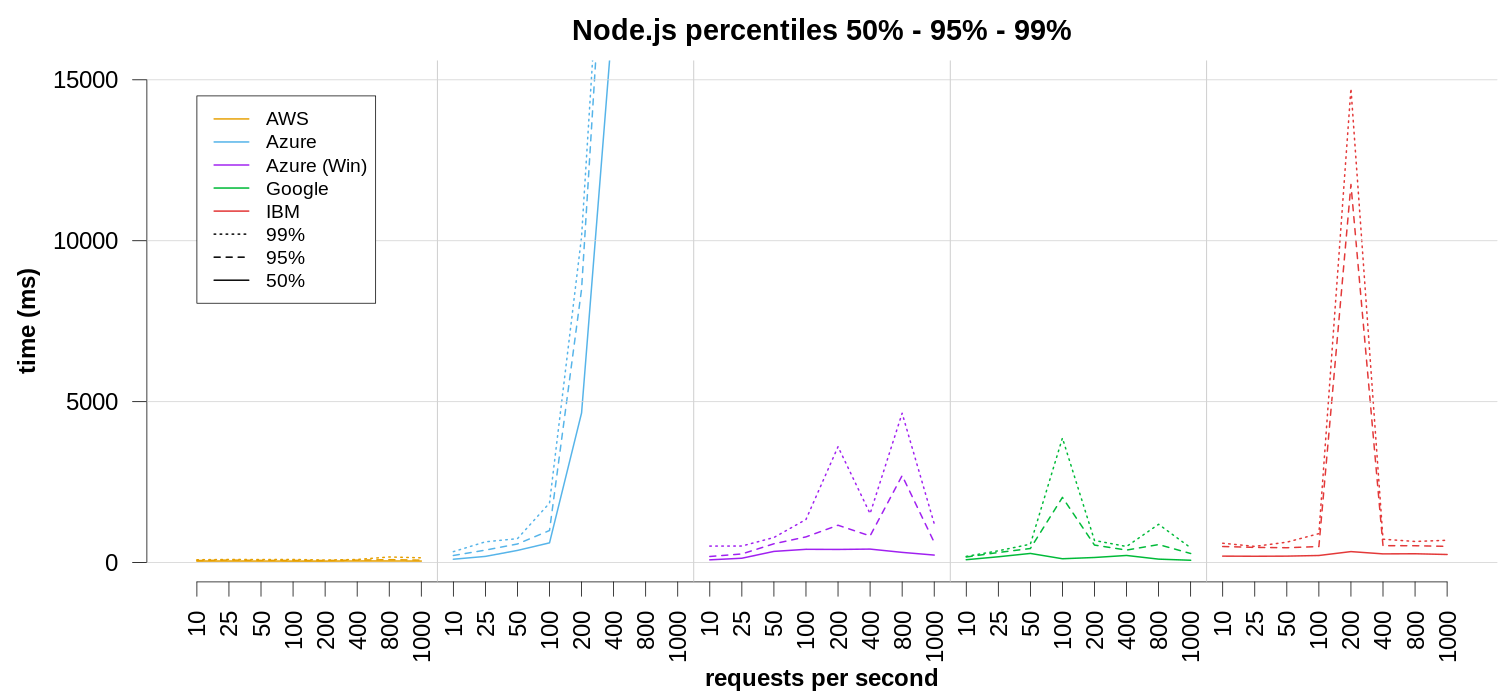
\includegraphics[width=1\textwidth]{bilder/plot_percentile_latency_node.png}
\captionsetup{justification=centering, labelfont=bf}
\caption[Latency percentiles (50\%, 95\%, 99\%) Node.js load test]{Latency percentiles (50\%, 95\%, 99\%) Node.js load test\\Source: illustration by author}
\label{fig:loadtest_percentile_node}
\end{center}
\end{figure}

\begin{figure}[b]
\begin{center}
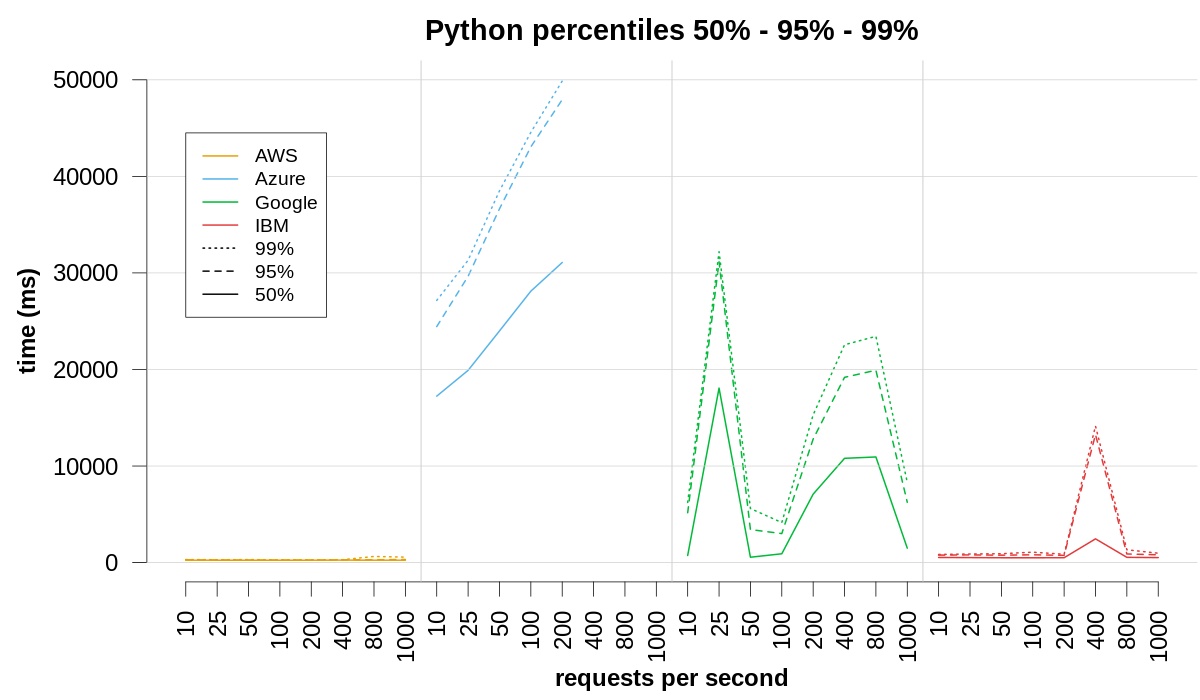
\includegraphics[width=1\textwidth]{bilder/plot_percentile_latency_python.png}
\captionsetup{justification=centering, labelfont=bf}
\caption[Latency percentiles (50\%, 95\%, 99\%) Python load test]{Latency percentiles (50\%, 95\%, 99\%) Python load test\\Source: illustration by author}
\label{fig:loadtest_percentile_python}
\end{center}
\end{figure}

\newpage

\begin{figure}[t]
\begin{center}
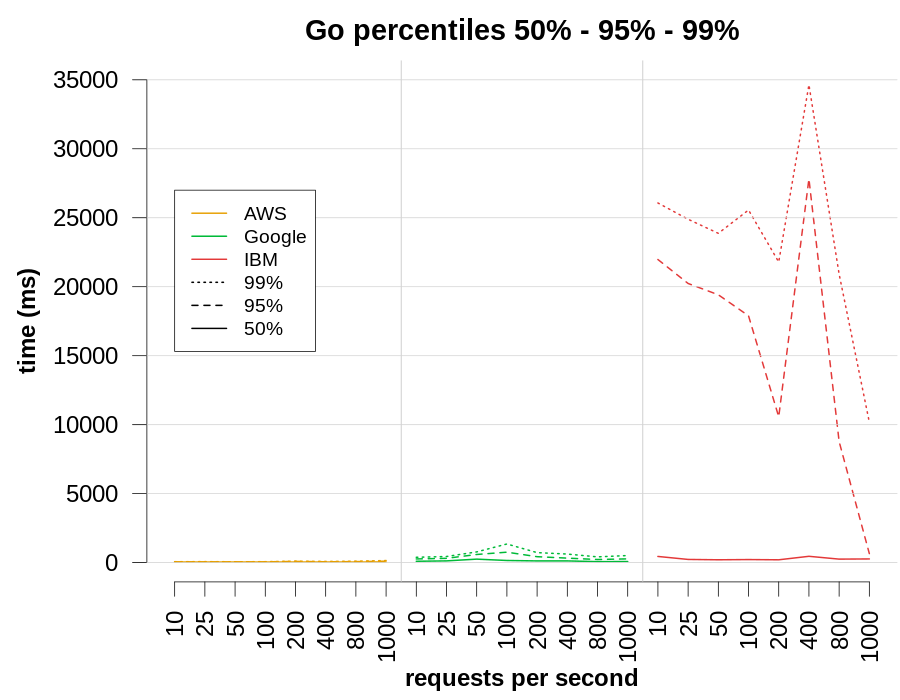
\includegraphics[width=0.75\textwidth]{bilder/plot_percentile_latency_go.png}
\captionsetup{justification=centering, labelfont=bf}
\caption[Latency percentiles (50\%, 95\%, 99\%) Go load test]{Latency percentiles (50\%, 95\%, 99\%) Go load test\\Source: illustration by author}
\label{fig:loadtest_percentile_go}
\end{center}
\end{figure}

\begin{figure}[b]
\begin{center}
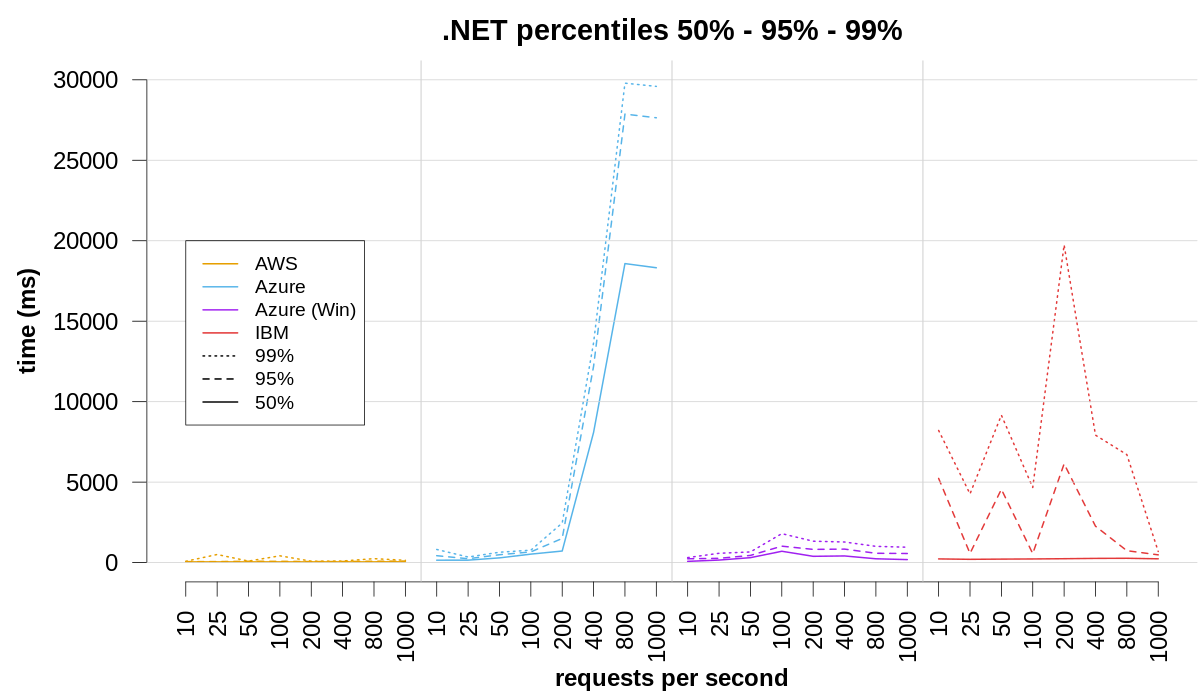
\includegraphics[width=0.95\textwidth]{bilder/plot_percentile_latency_dotnet.png}
\captionsetup{justification=centering, labelfont=bf}
\caption[Latency percentiles (50\%, 95\%, 99\%) .NET load test]{Latency percentiles (50\%, 95\%, 99\%) .NET load test\\Source: illustration by author}
\label{fig:loadtest_percentile_dotnet}
\end{center}
\end{figure}

\newpage

\begin{table}[b]
    \centering
    \begin{tabular}{|l|r|r|r|r|r|r|} \hline
    \textbf{Runtime} & \textbf{RPS (goal)} & \textbf{RPS (actual)} & \textbf{Avg.} & \textbf{50\%} & \textbf{95\%} & \textbf{99\%} \\ \hline
    Node.js	&	10	&	10	&	48ms	&	49ms	&	63ms	&	88ms	\\ \hline
Node.js	&	25	&	25	&	51ms	&	49ms	&	79ms	&	98ms	\\ \hline
Node.js	&	50	&	49	&	49ms	&	48ms	&	69ms	&	95ms	\\ \hline
Node.js	&	100	&	98	&	49ms	&	47ms	&	68ms	&	98ms	\\ \hline
Node.js	&	200	&	197	&	47ms	&	47ms	&	65ms	&	80ms	\\ \hline
Node.js	&	400	&	393	&	53ms	&	51ms	&	77ms	&	97ms	\\ \hline
Node.js	&	800	&	786	&	58ms	&	51ms	&	92ms	&	175ms	\\ \hline
Node.js	&	1000	&	979	&	53ms	&	48ms	&	77ms	&	149ms	\\ \hline
Python	&	10	&	10	&	255ms	&	252ms	&	293ms	&	315ms	\\ \hline
Python	&	25	&	25	&	249ms	&	247ms	&	273ms	&	300ms	\\ \hline
Python	&	50	&	50	&	248ms	&	246ms	&	269ms	&	310ms	\\ \hline
Python	&	100	&	98	&	249ms	&	247ms	&	267ms	&	289ms	\\ \hline
Python	&	200	&	197	&	249ms	&	247ms	&	268ms	&	288ms	\\ \hline
Python	&	400	&	393	&	257ms	&	257ms	&	285ms	&	299ms	\\ \hline
Python	&	800	&	785	&	263ms	&	251ms	&	298ms	&	638ms	\\ \hline
Python	&	1000	&	978	&	264ms	&	251ms	&	323ms	&	567ms	\\ \hline
Go	&	10	&	10	&	40ms	&	42ms	&	53ms	&	67ms	\\ \hline
Go	&	25	&	25	&	39ms	&	41ms	&	51ms	&	71ms	\\ \hline
Go	&	50	&	49	&	40ms	&	41ms	&	52ms	&	61ms	\\ \hline
Go	&	100	&	98	&	42ms	&	41ms	&	55ms	&	68ms	\\ \hline
Go	&	200	&	197	&	47ms	&	44ms	&	89ms	&	106ms	\\ \hline
Go	&	400	&	393	&	44ms	&	44ms	&	61ms	&	85ms	\\ \hline
Go	&	800	&	786	&	46ms	&	43ms	&	73ms	&	104ms	\\ \hline
Go	&	1000	&	977	&	56ms	&	47ms	&	103ms	&	151ms	\\ \hline
.NET	&	10	&	10	&	46ms	&	46ms	&	61ms	&	81ms	\\ \hline
.NET	&	25	&	25	&	50ms	&	45ms	&	63ms	&	504ms	\\ \hline
.NET	&	50	&	49	&	50ms	&	47ms	&	82ms	&	94ms	\\ \hline
.NET	&	100	&	98	&	56ms	&	47ms	&	79ms	&	422ms	\\ \hline
.NET	&	200	&	197	&	49ms	&	47ms	&	66ms	&	87ms	\\ \hline
.NET	&	400	&	393	&	49ms	&	46ms	&	68ms	&	99ms	\\ \hline
.NET	&	800	&	786	&	53ms	&	47ms	&	84ms	&	246ms	\\ \hline
.NET	&	1000	&	978	&	54ms	&	49ms	&	94ms	&	143ms	\\ \hline
    \end{tabular}
    \caption[AWS load test details]{AWS load test details. 50\% meaning that 50\% of the requests could been served in that time or less. Same applies for 95\% and 99\%.}
    \label{table:aws_load_test}
\end{table}

\begin{table}[h]
    \centering
    \begin{tabular}{|l|l|r|r|r|r|r|r|} \hline
    \textbf{OS} & \textbf{Runtime} & \textbf{RPS (goal)} & \textbf{RPS (actual)} & \textbf{Avg.} & \textbf{50\%} & \textbf{95\%} & \textbf{99\%} \\ \hline
Linux	&	Node.js	&	10	&	10	&	123ms	&	105ms	&	221ms	&	340ms	\\ \hline
Linux	&	Node.js	&	25	&	25	&	205ms	&	193ms	&	388ms	&	646ms	\\ \hline
Linux	&	Node.js	&	50	&	49	&	375ms	&	379ms	&	579ms	&	744ms	\\ \hline
Linux	&	Node.js	&	100	&	98	&	640ms	&	614ms	&	997ms	&	1850ms	\\ \hline
Linux	&	Node.js	&	200	&	179	&	4755ms	&	4650ms	&	8495ms	&	10130ms	\\ \hline
Linux	&	Node.js	&	400	&	227	&	16505ms	&	17190ms	&	24642ms	&	26100ms	\\ \hline
Linux	&	Node.js	&	800	&	278	&	23934ms	&	24480ms	&	37027ms	&	38700ms	\\ \hline
Linux	&	Node.js	&	1000	&	327	&	24218ms	&	24840ms	&	37388ms	&	39290ms	\\ \hline
Linux	&	Python	&	10	&	6	&	16498ms	&	17240ms	&	24444ms	&	27150ms	\\ \hline
Linux	&	Python	&	25	&	12	&	19444ms	&	19910ms	&	29655ms	&	31310ms	\\ \hline
Linux	&	Python	&	50	&	18	&	23427ms	&	23990ms	&	36635ms	&	38500ms	\\ \hline
Linux	&	Python	&	100	&	25	&	27261ms	&	28110ms	&	43057ms	&	44560ms	\\ \hline
Linux	&	Python	&	200	&	30	&	30448ms	&	31080ms	&	47940ms	&	49870ms	\\ \hline
Linux	&	Python	&	400	&	15	&	9365ms	&	8640ms	&	23167ms	&	28480ms	\\ \hline
Linux	&	Python	&	800	&	14	&	6949ms	&	5520ms	&	19382ms	&	23950ms	\\ \hline
Linux	&	Python	&	1000	&	15	&	7327ms	&	6170ms	&	19447ms	&	24670ms	\\ \hline
Linux	&	.NET	&	10	&	10	&	204ms	&	150ms	&	430ms	&	817ms	\\ \hline
Linux	&	.NET	&	25	&	25	&	157ms	&	152ms	&	241ms	&	347ms	\\ \hline
Linux	&	.NET	&	50	&	49	&	310ms	&	294ms	&	489ms	&	644ms	\\ \hline
Linux	&	.NET	&	100	&	98	&	515ms	&	527ms	&	665ms	&	772ms	\\ \hline
Linux	&	.NET	&	200	&	197	&	783ms	&	720ms	&	1502ms	&	2460ms	\\ \hline
Linux	&	.NET	&	400	&	324	&	8152ms	&	8090ms	&	12198ms	&	13660ms	\\ \hline
Linux	&	.NET	&	800	&	407	&	18140ms	&	18580ms	&	27869ms	&	29790ms	\\ \hline
Linux	&	.NET	&	1000	&	512	&	18012ms	&	18320ms	&	27640ms	&	29590ms	\\ \hline
Windows	&	Node.js	&	10	&	10	&	102ms	&	86ms	&	190ms	&	513ms	\\ \hline
Windows	&	Node.js	&	25	&	25	&	150ms	&	136ms	&	269ms	&	515ms	\\ \hline
Windows	&	Node.js	&	50	&	49	&	335ms	&	348ms	&	585ms	&	780ms	\\ \hline
Windows	&	Node.js	&	100	&	98	&	413ms	&	413ms	&	799ms	&	1340ms	\\ \hline
Windows	&	Node.js	&	200	&	197	&	515ms	&	409ms	&	1161ms	&	3600ms	\\ \hline
Windows	&	Node.js	&	400	&	393	&	436ms	&	420ms	&	829ms	&	1520ms	\\ \hline
Windows	&	Node.js	&	800	&	785	&	672ms	&	318ms	&	2703ms	&	4640ms	\\ \hline
Windows	&	Node.js	&	1000	&	979	&	282ms	&	234ms	&	630ms	&	1210ms	\\ \hline
Windows	&	.NET	&	10	&	10	&	99ms	&	77ms	&	238ms	&	311ms	\\ \hline
Windows	&	.NET	&	25	&	25	&	158ms	&	158ms	&	266ms	&	579ms	\\ \hline
Windows	&	.NET	&	50	&	49	&	277ms	&	307ms	&	447ms	&	662ms	\\ \hline
Windows	&	.NET	&	100	&	98	&	671ms	&	705ms	&	1022ms	&	1800ms	\\ \hline
Windows	&	.NET	&	200	&	197	&	423ms	&	391ms	&	822ms	&	1330ms	\\ \hline
Windows	&	.NET	&	400	&	393	&	433ms	&	414ms	&	839ms	&	1280ms	\\ \hline
Windows	&	.NET	&	800	&	786	&	274ms	&	238ms	&	580ms	&	1010ms	\\ \hline
Windows	&	.NET	&	1000	&	979	&	230ms	&	187ms	&	566ms	&	956ms	\\ \hline
    \end{tabular}
    \caption[Azure load test details]{Azure load test details. 50\% meaning that 50\% of the requests could been served in that time or less. Same applies for 95\% and 99\%.}
    \label{table:azure_load_test}
\end{table}

\newpage
\begin{table}[h]
    \centering
    \begin{tabular}{|l|r|r|r|r|r|r|} \hline
    \textbf{Runtime} & \textbf{RPS (goal)} & \textbf{RPS (actual)} & \textbf{Avg.} & \textbf{50\%} & \textbf{95\%} & \textbf{99\%} \\ \hline
Node.js	&	10	&	10	&	99ms	&	90ms	&	131ms	&	193ms	\\ \hline
Node.js	&	25	&	25	&	183ms	&	181ms	&	242ms	&	367ms	\\ \hline
Node.js	&	50	&	50	&	265ms	&	285ms	&	339ms	&	572ms	\\ \hline
Node.js	&	100	&	99	&	362ms	&	120ms	&	208ms	&	3870ms	\\ \hline
Node.js	&	200	&	197	&	211ms	&	159ms	&	265ms	&	688ms	\\ \hline
Node.js	&	400	&	393	&	228ms	&	222ms	&	291ms	&	500ms	\\ \hline
Node.js	&	800	&	786	&	181ms	&	108ms	&	182ms	&	1190ms	\\ \hline
Node.js	&	1000	&	978	&	113ms	&	73ms	&	147ms	&	460ms	\\ \hline
Python	&	10	&	10	&	1356ms	&	740ms	&	1240ms	&	6230ms	\\ \hline
Python	&	25	&	12	&	18448ms	&	18070ms	&	24560ms	&	32190ms	\\ \hline
Python	&	50	&	49	&	915ms	&	557ms	&	918ms	&	5600ms	\\ \hline
Python	&	100	&	98	&	1200ms	&	914ms	&	1590ms	&	4150ms	\\ \hline
Python	&	200	&	168	&	7315ms	&	7090ms	&	9630ms	&	15300ms	\\ \hline
Python	&	400	&	297	&	10871ms	&	10800ms	&	14300ms	&	22560ms	\\ \hline
Python	&	800	&	575	&	11144ms	&	10940ms	&	14680ms	&	23430ms	\\ \hline
Python	&	1000	&	976	&	2246ms	&	1500ms	&	3360ms	&	8310ms	\\ \hline
Go	&	10	&	10	&	113ms	&	97ms	&	122ms	&	386ms	\\ \hline
Go	&	25	&	25	&	138ms	&	125ms	&	164ms	&	442ms	\\ \hline
Go	&	50	&	49	&	271ms	&	252ms	&	350ms	&	776ms	\\ \hline
Go	&	100	&	98	&	241ms	&	154ms	&	265ms	&	1350ms	\\ \hline
Go	&	200	&	197	&	172ms	&	123ms	&	212ms	&	724ms	\\ \hline
Go	&	400	&	393	&	151ms	&	124ms	&	178ms	&	620ms	\\ \hline
Go	&	800	&	786	&	98ms	&	70ms	&	124ms	&	416ms	\\ \hline
Go	&	1000	&	979	&	131ms	&	78ms	&	140ms	&	512ms	\\ \hline
    \end{tabular}
    \caption[Google load test details]{Google load test details. 50\% meaning that 50\% of the requests could been served in that time or less. Same applies for 95\% and 99\%.}
    \label{table:google_load_test}
\end{table}


\newpage
\begin{table}[h]
    \centering
    \begin{tabular}{|l|r|r|r|r|r|r|} \hline
    \textbf{Runtime} & \textbf{RPS (goal)} & \textbf{RPS (actual)} & \textbf{Avg.} & \textbf{50\%} & \textbf{95\%} & \textbf{99\%} \\ \hline
Node.js	&	10	&	10	&	289ms	&	201ms	&	500ms	&	602ms	\\ \hline
Node.js	&	25	&	25	&	259ms	&	197ms	&	473ms	&	504ms	\\ \hline
Node.js	&	50	&	50	&	252ms	&	201ms	&	462ms	&	635ms	\\ \hline
Node.js	&	100	&	98	&	280ms	&	221ms	&	499ms	&	900ms	\\ \hline
Node.js	&	200	&	197	&	2707ms	&	342ms	&	11747ms	&	14730ms	\\ \hline
Node.js	&	400	&	393	&	313ms	&	271ms	&	526ms	&	727ms	\\ \hline
Node.js	&	800	&	784	&	293ms	&	275ms	&	524ms	&	657ms	\\ \hline
Node.js	&	1000	&	978	&	277ms	&	252ms	&	505ms	&	694ms	\\ \hline
Python	&	10	&	10	&	565ms	&	531ms	&	774ms	&	845ms	\\ \hline
Python	&	25	&	25	&	563ms	&	518ms	&	798ms	&	891ms	\\ \hline
Python	&	50	&	49	&	536ms	&	503ms	&	769ms	&	921ms	\\ \hline
Python	&	100	&	98	&	545ms	&	502ms	&	809ms	&	1080ms	\\ \hline
Python	&	200	&	197	&	527ms	&	505ms	&	751ms	&	866ms	\\ \hline
Python	&	400	&	382	&	4640ms	&	2460ms	&	13255ms	&	14140ms	\\ \hline
Python	&	800	&	781	&	593ms	&	545ms	&	894ms	&	1330ms	\\ \hline
Python	&	1000	&	977	&	547ms	&	518ms	&	809ms	&	973ms	\\ \hline
Go	&	10	&	10	&	5296ms	&	447ms	&	21971ms	&	26070ms	\\ \hline
Go	&	25	&	21	&	3600ms	&	230ms	&	20234ms	&	24890ms	\\ \hline
Go	&	50	&	50	&	3373ms	&	205ms	&	19415ms	&	23870ms	\\ \hline
Go	&	100	&	98	&	2731ms	&	221ms	&	17891ms	&	25560ms	\\ \hline
Go	&	200	&	198	&	1331ms	&	204ms	&	10568ms	&	21790ms	\\ \hline
Go	&	400	&	390	&	7027ms	&	457ms	&	27820ms	&	34640ms	\\ \hline
Go	&	800	&	777	&	1222ms	&	253ms	&	8774ms	&	20910ms	\\ \hline
Go	&	1000	&	979	&	498ms	&	266ms	&	654ms	&	10180ms	\\ \hline
.NET	&	10	&	10	&	848ms	&	230ms	&	5231ms	&	8210ms	\\ \hline
.NET	&	25	&	25	&	380ms	&	204ms	&	571ms	&	4270ms	\\ \hline
.NET	&	50	&	49	&	717ms	&	217ms	&	4555ms	&	9160ms	\\ \hline
.NET	&	100	&	94	&	391ms	&	227ms	&	559ms	&	4670ms	\\ \hline
.NET	&	200	&	196	&	1121ms	&	242ms	&	6136ms	&	19740ms	\\ \hline
.NET	&	400	&	393	&	616ms	&	262ms	&	2263ms	&	7920ms	\\ \hline
.NET	&	800	&	785	&	488ms	&	269ms	&	741ms	&	6710ms	\\ \hline
.NET	&	1000	&	978	&	263ms	&	236ms	&	482ms	&	691ms	\\ \hline
    \end{tabular}
    \caption[IBM load test details]{IBM load test details. 50\% meaning that 50\% of the requests could been served in that time or less. Same applies for 95\% and 99\%.}
    \label{table:ibm_load_test}
\end{table}


\chapter{Miscellaneous}

\begin{lstlisting}[frame=single,caption={Google Cloud Functions - Example content of \texttt{/proc/cpuinfo}},label=lst:cpuinfo]
processor       : 0
vendor_id       : GenuineIntel
cpu family      : 6
model           : 85
model name      : unknown
stepping        : unknown
cpu MHz         : 2000.162
fpu             : yes
fpu_exception   : yes
cpuid level     : 13
wp              : yes
flags           :
bogomips        : 2000.16
clflush size    : 64
cache_alignment : 64
address sizes   : 46 bits physical, 48 bits virtual
power management:
\end{lstlisting}

\begin{lstlisting}[frame=single,caption={IBM Cloud Functions - Example content of \texttt{/proc/cpuinfo}},label=lst:cpuinfo2]
processor       : [0..3]
vendor_id       : GenuineIntel
cpu family      : 6
model           : 63
model name      : Intel(R) Xeon(R) CPU E5-2683 v3 @ 2.00GHz
stepping        : 2
microcode       : 0x43
cpu MHz         : 2000.056
cache size      : 35840 KB
physical id     : 0
siblings        : 4
core id         : 0
cpu cores       : 4
apicid          : 0
initial apicid  : 0
fpu             : yes
fpu_exception   : yes
cpuid level     : 13
wp              : yes
flags           : 
bugs            : cpu_meltdown spectre_v1 spectre_v2 spec_store_bypass l1tf mds swapgs
bogomips        : 4000.11
clflush size    : 64
cache_alignment : 64
address sizes   : 46 bits physical, 48 bits virtual
power management:
\end{lstlisting}